\documentclass{report}
\usepackage[T1]{fontenc}
\usepackage[utf8]{inputenc}

\usepackage{amsmath}
\usepackage{biblatex}
\usepackage{fancyvrb}
\usepackage{fontspec}
\usepackage[margin=1.5in,a4paper]{geometry}
\usepackage[hidelinks]{hyperref}
\usepackage{microtype}
\usepackage{pgfplots}
\pgfplotsset{compat=1.7}
\usepackage{siunitx}
\usepackage{subcaption}
\usepackage{tikz}
\usetikzlibrary{arrows, fit, positioning, quotes}
\usepackage{titlesec}
\usepackage{titling}

\setmainfont{Linux Libertine}
\setsansfont[Scale=0.9]{Open Sans}
\setmonofont[Scale=0.9]{Inconsolata}
\newfontfamily\headfamily[]{Chicago}
\titleformat*{\section}{\Large\headfamily}
\titleformat*{\subsection}{\large\headfamily}
\titleformat*{\subsubsection}{\large\headfamily}
\renewcommand{\maketitlehooka}{\headfamily}

\newcommand{\setb}[1]{\left\{ #1 \right\}}
\newcommand{\q}[1]{\mathsf{#1}}
\newcommand{\todo}[1]{\textbf{TODO: #1}}
\newcommand{\dontcare}{\#}

\addbibresource{games.bib}

\widowpenalty=500
\clubpenalty=500

\begin{document}
\title{Platypus Games Without Frontiers}
\author{Hayley Patton}
\date{\today}
\maketitle

\tableofcontents

\chapter{Introduction}

The aim of this project is to run a complete tournament
of the Platypus game, which has been stated to be infeasible
by my supervisor James Harland in his lectures for the
Computing Theory course.
The Platypus game is related to the \emph{busy beaver} game,
which aims to find the Turing machine of a given complexity
which generates the longest string on a tape and eventually halts.
But the Platypus game is difficult to run for different reasons: it
involves a finite and cyclic board rather than an infinite tape, and
the length of a Platypus game can run is bounded, but the search space
is much larger due to the Platypus game involving two competing
machines sharing the board.

\section{The Platypus game}

The \emph{Platypus} game is is a theoretical game introduced in the
Computing Theory course in RMIT, used to teach automata
(particularly Turing machines) and complexity theory.
The Platypus game is played by two 4-state Turing machine
\emph{players}, which share a two-symbol board with 21 cells. The states
are named Kangaroo, Emu, Wombat and Platypus, and the symbols
are named Yellow and Green. (These names are sometimes shortened
to their initials for brevity.) One such machine is represented in three
different ways in Figure~\ref{fig:representations}. Note that a transition
% In unrelated conversation I hear "graphical representation" more, but
% I interpret it first as "visual" and then realise it means "using a graph".
is written in the graph representation as $S_1 \rightarrow S_2, D$ where
$S_1$ is the symbol read, $S_2$ the symbol written and $D$ the direction
to move in. The board is initially all Yellow.

All machines start in the Kangaroo state, and the game ends when
both players have made 50 moves each, or a player with a Platypus
state reads a Green cell.
Players earn points in a game by changing the colours of cells; the
winner has the most points.

\begin{figure}
  \begin{center}
    \begin{tabular}{rr|ccccccc}
      \hline
      From & Colour & Y & G & Y & G & Y & G & Y \\
      & Animal & K & K & E & E & W & W & P \\
      \hline
      To & Colour & G & Y & G & G & G & Y & G \\
      & Animal & W & K & W & E & E & E & K \\
      & Direction & G & G & G & G & W & G & G \\
      \hline
      \multicolumn{2}{r}{Hexadecimal} &
      \texttt{A} & \texttt{F} & \texttt{A} & \texttt{C} & \texttt{4} & \texttt{D} & \texttt{E}
    \end{tabular}
    
    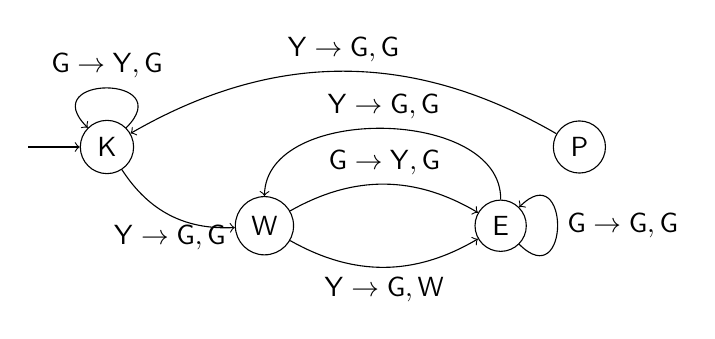
\begin{tikzpicture}
      \node[draw, circle] (P) at (6, 0) {\sffamily P};
      \node[draw, circle] (W) at (2, -1) {\sffamily W};
      \node[draw, circle] (E) at (5, -1) {\sffamily E};
      \node[draw, circle] (K) at (0, 0) {\sffamily K};
      \draw[->] (-1, 0) to (K);
      \draw[->] (P) to[bend right] node[midway, above] {$\q{Y} \rightarrow \q{G}, \q{G}$} (K);
      \draw[->] (W) to[bend left] node[midway, above] {$\q{G} \rightarrow \q{Y}, \q{G}$} (E);
      \draw[->] (W) to[bend right] node[midway, below] {$\q{Y} \rightarrow \q{G}, \q{W}$} (E);
      \draw[->] (E) to[in=45, out=-45, looseness=5] node[midway, right] {$\q{G} \rightarrow \q{G}, \q{G}$} (E);
      \draw[->] (E) to[bend right=90] node[midway, above] {$\q{Y} \rightarrow \q{G}, \q{G}$} (W);
      \draw[->] (K) to[in=135, out=45, looseness=5] node[midway, above] {$\q{G} \rightarrow \q{Y}, \q{G}$} (K);
      \draw[->] (K) to[bend right] node[midway, below] {$\q{Y} \rightarrow \q{G}, \q{G}$} (W);
    \end{tikzpicture}
  \end{center}
  \caption{A Platypus machine represented in three different ways.}
  \label{fig:representations}
\end{figure}

\section{The Platypus tournament}

A Platypus \emph{tournament} may be played, to find a machine
out of some set of machines which wins the most matches (or
earns the most points in total, if multiple machines win the
same largest number of matches). A tournament involves playing
every player against every player, including matches
with machines playing themselves and matches which have the
players reversed to other matches; a tournament of $n$ matches
thus involves playing $n^2$ matches%
\footnote{The Computing Theory course defines a match between
  machines $a$ and $b$ to be playing a Platypus game with players
  $a$ and $b$, and another game with players $b$ and $a$. This
  definition would have $\frac12 n(n-1)$ matches, as the outcome of
  a match does not depend on the order the machines. 
  It is however useful to separate the two times the game is played
  (and I analyse them separately in \autoref{chap:results}), so I
  define a match to be playing just one game, and the result of
  a match does depend on the order of the machines.}
The \emph{complete tournament} involves playing every possible
matches with every possible machine, of which there are $2^{56}$
(approximately 72 quadrillion) matches. If one could run 1 billion
Platypus matches per second, they would still need 2.3 years to
run every possible match.

It is interesting to compare the effort of running a complete
tournament to performing a brute-force attack on the insecure
\emph{Data Encryption Standard} (DES) encryption algorithm, which
has $2^{56}$ possible keys. The \emph{Deep Crack} machine built by the
Electronic Frontier Foundation used less than US\$250,000 of custom
hardware to search the entire key space in about nine days, testing
88 billion keys per second \cite{deep-crack}. A more recent system using
\emph{field-programmable gate arrays} can search 768 billion keys per
second, searching the entire key space in 26 hours \cite{crack.sh}. But the
Platypus game is not an encryption algorithm, so the amount of
effort can (more easily) be reduced by analysis of the Platypus game.
The result of a Platypus tournament contains more data than
which key correctly decrypts a message however, and Platypus matches
have variable lengths (whereas DES encryption takes constant time with
regards to the key), so parallelisation is more difficult.

Thus the project requires both high-level and low-level optimisations,
which I found very interesting. The number of matches can be
reduced by a factor $25\times$ by eliminating equivalent machines
(as in Chapter 2), and the remaining machines must be tested with
high throughput (for which I eventually settled on GPGPU with cloud
computing, as described in Chapter 3). I was then able to run the full
tournament in nine days.

\section{Representing Platypus machines}
\label{sec:representation}

A computer program requires a concrete representation of the abstract
concept of a Platypus machine, in order to use the machine.
There are some desirable properties of a representation:

\begin{itemize}
\item It should be easy to iterate all the possible Platypus machines.
\item Finding a transition by input to the transition function should be fast.%
\item The representation should be compact, to allow for fitting many
  machines in memory.
\end{itemize}

I represent a Platypus machine as an integer in the range
$[0, 2^{28})$. The 28 bits of a machine are divided between its seven
defined 4-bit transitions; each 4-bit transition is comprised of
1 bit for the symbol written by the player (Green or Yellow), 2 bits
for the state to transition to (Platypus, Wombat, Emu or Kangaroo),
and 1 bit for the direction that the player moves (towards the wattle
or the ghost gum).

The mapping between each abstract value used by the machine and
concrete values used by an implementation is ultimately arbitrary. I
use a mapping which allows using the indexes of the tabular format used
in the course material for Computing Theory, as presented in
Figure~\ref{fig:representations}. Green is represented as 0, and Yellow as 1;
and a Platypus is represented as 0, Wombat as 1, Emu as 2, and Kangaroo
as 3. The transition for reading a cell of colour $c$ with animal $a$
starts from the $4(2a + c - 1)$th bit (starting at 0). Note that the transition
for reading a Green cell as Platypus starts at the $-4$th bit as $a = 0$ and
$c = 0$, but we will never perform a transition in that situation.

The representation provides all the desired properties:

\begin{itemize}
\item All machines may be iterated over by producing successive
  integers, which is trivial.
\item A transition may be found by extracting a sequence of bits from
  the integer, which is very fast. The Common Lisp language \cite{common-lisp}
  provides the functions \texttt{ldb} (``load byte'') and
  \texttt{dpb} (``deposit byte'') for extracting and replacing sequences
  of bits from integers; I use these functions extensively in my implementation.
\item The representation is an \emph{implicit data structure}
  \cite{implicit-data-structures}, requiring the minimum necessary
  number of bits to encode a machine; Common Lisp implementations
  also do not perform heap allocations for small integers (``fixnums'').
\end{itemize}

Additionally, a machine using the representation may be efficiently
updated by replacing part of an integer; this update does not modify
the original machine, allowing for a functional programming style
while constructing and modifying machines while detecting
equivalences. This representation is implemented in the file
\texttt{Code/representation.lisp}.

\section{Conventions}

The real time taken to perform computations was measured on my
desktop, which has a 12-core/24-thread Ryzen 5900X processor with 16GB
of memory, and a RX 580 graphics card with 8GB of memory. I report
many durations in \emph{CPU-seconds} -- the sum of all times taken
by each core -- as many problems are run across all cores.

\section{Infrastructure}

The code and {\fontfamily{lmr}\selectfont \LaTeX} sources for this report
are hosted on GitHub at \url{https://github.com/no-defun-allowed/platypus-games-without-frontiers/}.
The code is predominantly written in Common Lisp, using some
extensions specific to the Steel Bank Common
Lisp\footnote{\url{http://sbcl.org/}} implementation. The GPGPU code is
written using Python, OpenCL and the PyOpenCL library.
I use cloud compute provided by the RMIT AWS Cloud Supercomputing
(RACE) Hub.
\chapter{Detecting equivalences}

Sheer throughput might not be sufficient to perform a full Platypus
tournament in a reasonable time frame. Even if we could run one billion
matches per second, we would still require approximately 2.3 years to run
all $2^{56}$ matches in the full tournament.

Baker \cite{triangle} discusses the optimisation of a brute force problem,
which makes many calls to a pure function with the same arguments.
He notes that \emph{memoisation} -- caching the results of an
expensive function call instead of recomputing the results -- allows
``one processor [to simulate] the execution of many processes with a single
execution''. But we never run a game between the exact same machines
more than once, so memoisation per se would not be effective.

We could still use the same principle if we could detect machines
which are \emph{equivalent} in a more abstract sense: two machines
are equivalent if they behave identically when faced against the same
opponent. We may then use knowledge of such equivalence to reduce the
number of matches played: the results of a match between machines $m_1$ and
$m_2$ must be identical to the results of a match between machines $m_3$
and $m_2$ if $m_1$ and $m_3$ are equivalent.
Exploiting such equivalences can provide a substantial speedup as the Platypus
tournament plays every machine against every machine, so reducing the
number of machines by some factor $f$ reduces the number of necessary
games to play by a factor $f^2$.

All the algorithms are implemented in the file \texttt{Code/equivalences.lisp}.
Generation of diagrams is implemented in the file \texttt{Code/report-diagrams.lisp}.

\section{Dead code elimination}

Consider the machines depicted in Figure~\ref{fig:dead-states}.
Both machines always move towards the ghost gum and turn
all cells Yellow, and thus the machines are equivalent, despite
five of the seven transitions being different. Any
configuration of these five transitions cannot affect the behaviour
of the machine, as there is no way for the machine to perform
these transitions. There are $(2^4)^5 = 1048576$ machines in total
which are equivalent to either machine, and we would prefer
to avoid running matches involving all of these machines. We
may use a \emph{dead code elimination} algorithm to normalise
all these machines to just one machine.

\begin{figure}
  \begin{center}
    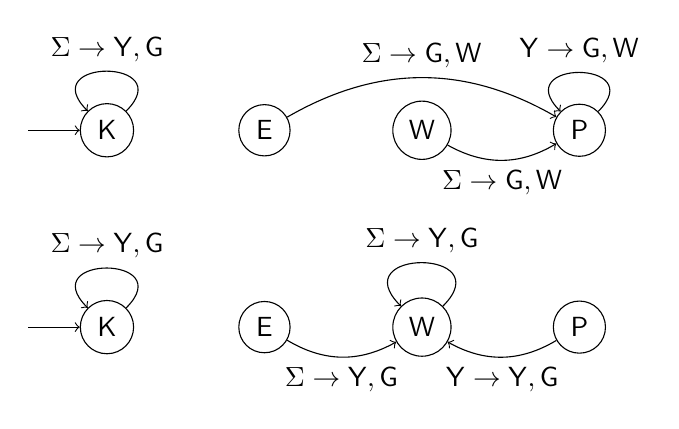
\begin{tikzpicture}
      \node[draw, circle] (P1) at (6, 0) {\sffamily P};
      \node[draw, circle] (W1) at (4, 0) {\sffamily W};
      \node[draw, circle] (E1) at (2, 0) {\sffamily E};
      \node[draw, circle] (K1) at (0, 0) {\sffamily K};
      \draw[->] (-1, 0) to (K1);
      \draw[->] (P1) to[in=135, out=45, looseness=5] node[midway, above] {$\q{Y} \rightarrow \q{G}, \q{W}$} (P1);
      \draw[->] (W1) to[bend right] node[midway, below] {$\Sigma \rightarrow \q{G}, \q{W}$} (P1);
      \draw[->] (E1) to[bend left] node[midway, above] {$\Sigma \rightarrow \q{G}, \q{W}$} (P1);
      \draw[->] (K1) to[in=135, out=45, looseness=5] node[midway, above] {$\Sigma \rightarrow \q{Y}, \q{G}$} (K1);
    
      \node[draw, circle] (P2) at (6, -2.5) {\sffamily P};
      \node[draw, circle] (W2) at (4, -2.5) {\sffamily W};
      \node[draw, circle] (E2) at (2, -2.5) {\sffamily E};
      \node[draw, circle] (K2) at (0, -2.5) {\sffamily K};
      \draw[->] (-1, -2.5) to (K2);
      \draw[->] (P2) to[bend left] node[midway, below] {$\q{Y} \rightarrow \q{Y}, \q{G}$} (W2);
      \draw[->] (W2) to[in=135, out=45, looseness=5] node[midway, above] {$\Sigma \rightarrow \q{Y}, \q{G}$} (W2);
      \draw[->] (E2) to[bend right] node[midway, below] {$\Sigma \rightarrow \q{Y}, \q{G}$} (W2);
      \draw[->] (K2) to[in=135, out=45, looseness=5] node[midway, above] {$\Sigma \rightarrow \q{Y}, \q{G}$} (K2);
    \end{tikzpicture}
  \end{center}
  \caption{Two equivalent machines (\texttt{\#xFF00000} and \texttt{\#xFFBBBBB}).}
  \label{fig:dead-states}
\end{figure}

A state is considered \emph{live} if it is either the initial state
state (the Kangaroo state in the Platypus game), or can be entered by
transitioning from another live state. All other states are \emph{dead}.
The transitions from a dead state cannot influence the behaviour
of a Platypus machine, as the machine cannot possibly transition
to a dead state. I traverse the transitions of the machine starting from
the Kangaroo state and copy transitions to another machine, leaving
all the transitions from unreachable states unset. 

108,988,816 unique machines (40.6\%) remain after dead code elimination.
The results are presented as a heatmap of unique machines after
deduplication in Figure~\ref{fig:dce}, with the X and Y axes having
different animals to transition to from the Kangaroo and Emu
states respectively. Almost no machines with only the Kangaroo state
live (the white stripe on the right) or only just the Kangaroo and
Emu states live remain. It took 109 CPU-seconds to eliminate
dead code from every Platypus machine.


\begin{figure}
  \begin{center}
    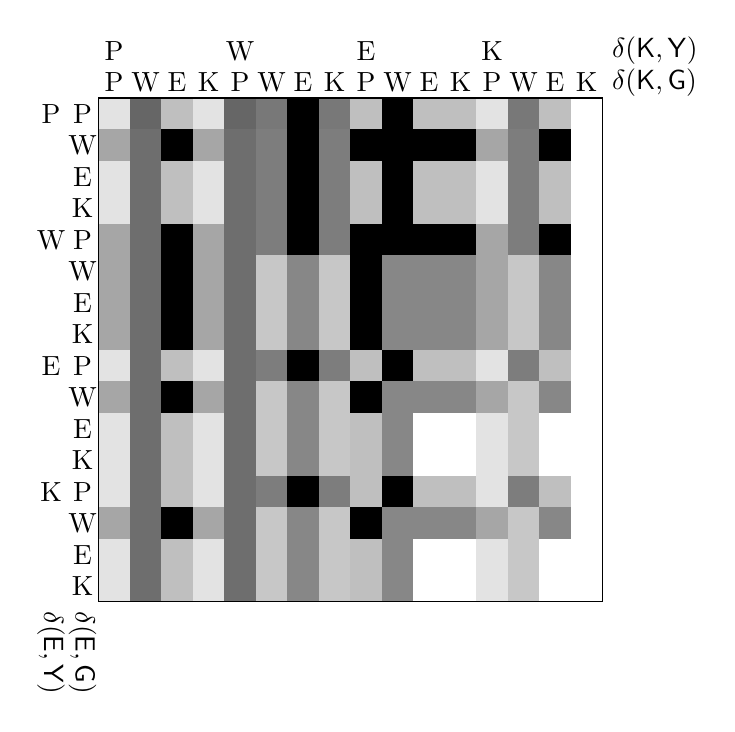
\begin{tikzpicture}[yscale=-1, scale=0.4]
  \node[anchor=west] at (16, -1.5) {$\delta (\q{K}, \q{Y})$};
  \node[anchor=west] at (16, -0.5) {$\delta (\q{K}, \q{G})$};
  \node[anchor=west, rotate=-90] at (-1.5, 16) {$\delta (\q{E}, \q{Y})$};
  \node[anchor=west, rotate=-90] at (-0.5, 16) {$\delta (\q{E}, \q{G})$};
  \node at (0.5, -1.5) {P}; \node at (-1.5, 0.5) {P};
  \node at (0.5, -0.5) {P}; \node at (-0.5, 0.5) {P};
  \node at (4.5, -0.5) {P}; \node at (-0.5, 4.5) {P};
  \node at (8.5, -0.5) {P}; \node at (-0.5, 8.5) {P};
  \node at (12.5, -0.5) {P}; \node at (-0.5, 12.5) {P};
  \node at (4.5, -1.5) {W}; \node at (-1.5, 4.5) {W};
  \node at (1.5, -0.5) {W}; \node at (-0.5, 1.5) {W};
  \node at (5.5, -0.5) {W}; \node at (-0.5, 5.5) {W};
  \node at (9.5, -0.5) {W}; \node at (-0.5, 9.5) {W};
  \node at (13.5, -0.5) {W}; \node at (-0.5, 13.5) {W};
  \node at (8.5, -1.5) {E}; \node at (-1.5, 8.5) {E};
  \node at (2.5, -0.5) {E}; \node at (-0.5, 2.5) {E};
  \node at (6.5, -0.5) {E}; \node at (-0.5, 6.5) {E};
  \node at (10.5, -0.5) {E}; \node at (-0.5, 10.5) {E};
  \node at (14.5, -0.5) {E}; \node at (-0.5, 14.5) {E};
  \node at (12.5, -1.5) {K}; \node at (-1.5, 12.5) {K};
  \node at (3.5, -0.5) {K}; \node at (-0.5, 3.5) {K};
  \node at (7.5, -0.5) {K}; \node at (-0.5, 7.5) {K};
  \node at (11.5, -0.5) {K}; \node at (-0.5, 11.5) {K};
  \node at (15.5, -0.5) {K}; \node at (-0.5, 15.5) {K};
  \fill[black!11!white] (0, 0) rectangle +(1, 1);
  \fill[black!35!white] (0, 1) rectangle +(1, 1);
  \fill[black!11!white] (0, 2) rectangle +(1, 1);
  \fill[black!11!white] (0, 3) rectangle +(1, 1);
  \fill[black!35!white] (0, 4) rectangle +(1, 1);
  \fill[black!35!white] (0, 5) rectangle +(1, 1);
  \fill[black!35!white] (0, 6) rectangle +(1, 1);
  \fill[black!35!white] (0, 7) rectangle +(1, 1);
  \fill[black!11!white] (0, 8) rectangle +(1, 1);
  \fill[black!35!white] (0, 9) rectangle +(1, 1);
  \fill[black!11!white] (0, 10) rectangle +(1, 1);
  \fill[black!11!white] (0, 11) rectangle +(1, 1);
  \fill[black!11!white] (0, 12) rectangle +(1, 1);
  \fill[black!35!white] (0, 13) rectangle +(1, 1);
  \fill[black!11!white] (0, 14) rectangle +(1, 1);
  \fill[black!11!white] (0, 15) rectangle +(1, 1);
  \fill[black!60!white] (1, 0) rectangle +(1, 1);
  \fill[black!57!white] (1, 1) rectangle +(1, 1);
  \fill[black!57!white] (1, 2) rectangle +(1, 1);
  \fill[black!57!white] (1, 3) rectangle +(1, 1);
  \fill[black!57!white] (1, 4) rectangle +(1, 1);
  \fill[black!57!white] (1, 5) rectangle +(1, 1);
  \fill[black!57!white] (1, 6) rectangle +(1, 1);
  \fill[black!57!white] (1, 7) rectangle +(1, 1);
  \fill[black!57!white] (1, 8) rectangle +(1, 1);
  \fill[black!57!white] (1, 9) rectangle +(1, 1);
  \fill[black!57!white] (1, 10) rectangle +(1, 1);
  \fill[black!57!white] (1, 11) rectangle +(1, 1);
  \fill[black!57!white] (1, 12) rectangle +(1, 1);
  \fill[black!57!white] (1, 13) rectangle +(1, 1);
  \fill[black!57!white] (1, 14) rectangle +(1, 1);
  \fill[black!57!white] (1, 15) rectangle +(1, 1);
  \fill[black!25!white] (2, 0) rectangle +(1, 1);
  \fill[black!100!white] (2, 1) rectangle +(1, 1);
  \fill[black!25!white] (2, 2) rectangle +(1, 1);
  \fill[black!25!white] (2, 3) rectangle +(1, 1);
  \fill[black!100!white] (2, 4) rectangle +(1, 1);
  \fill[black!100!white] (2, 5) rectangle +(1, 1);
  \fill[black!100!white] (2, 6) rectangle +(1, 1);
  \fill[black!100!white] (2, 7) rectangle +(1, 1);
  \fill[black!25!white] (2, 8) rectangle +(1, 1);
  \fill[black!100!white] (2, 9) rectangle +(1, 1);
  \fill[black!25!white] (2, 10) rectangle +(1, 1);
  \fill[black!25!white] (2, 11) rectangle +(1, 1);
  \fill[black!25!white] (2, 12) rectangle +(1, 1);
  \fill[black!100!white] (2, 13) rectangle +(1, 1);
  \fill[black!25!white] (2, 14) rectangle +(1, 1);
  \fill[black!25!white] (2, 15) rectangle +(1, 1);
  \fill[black!11!white] (3, 0) rectangle +(1, 1);
  \fill[black!35!white] (3, 1) rectangle +(1, 1);
  \fill[black!11!white] (3, 2) rectangle +(1, 1);
  \fill[black!11!white] (3, 3) rectangle +(1, 1);
  \fill[black!35!white] (3, 4) rectangle +(1, 1);
  \fill[black!35!white] (3, 5) rectangle +(1, 1);
  \fill[black!35!white] (3, 6) rectangle +(1, 1);
  \fill[black!35!white] (3, 7) rectangle +(1, 1);
  \fill[black!11!white] (3, 8) rectangle +(1, 1);
  \fill[black!35!white] (3, 9) rectangle +(1, 1);
  \fill[black!11!white] (3, 10) rectangle +(1, 1);
  \fill[black!11!white] (3, 11) rectangle +(1, 1);
  \fill[black!11!white] (3, 12) rectangle +(1, 1);
  \fill[black!35!white] (3, 13) rectangle +(1, 1);
  \fill[black!11!white] (3, 14) rectangle +(1, 1);
  \fill[black!11!white] (3, 15) rectangle +(1, 1);
  \fill[black!60!white] (4, 0) rectangle +(1, 1);
  \fill[black!57!white] (4, 1) rectangle +(1, 1);
  \fill[black!57!white] (4, 2) rectangle +(1, 1);
  \fill[black!57!white] (4, 3) rectangle +(1, 1);
  \fill[black!57!white] (4, 4) rectangle +(1, 1);
  \fill[black!57!white] (4, 5) rectangle +(1, 1);
  \fill[black!57!white] (4, 6) rectangle +(1, 1);
  \fill[black!57!white] (4, 7) rectangle +(1, 1);
  \fill[black!57!white] (4, 8) rectangle +(1, 1);
  \fill[black!57!white] (4, 9) rectangle +(1, 1);
  \fill[black!57!white] (4, 10) rectangle +(1, 1);
  \fill[black!57!white] (4, 11) rectangle +(1, 1);
  \fill[black!57!white] (4, 12) rectangle +(1, 1);
  \fill[black!57!white] (4, 13) rectangle +(1, 1);
  \fill[black!57!white] (4, 14) rectangle +(1, 1);
  \fill[black!57!white] (4, 15) rectangle +(1, 1);
  \fill[black!53!white] (5, 0) rectangle +(1, 1);
  \fill[black!51!white] (5, 1) rectangle +(1, 1);
  \fill[black!51!white] (5, 2) rectangle +(1, 1);
  \fill[black!51!white] (5, 3) rectangle +(1, 1);
  \fill[black!51!white] (5, 4) rectangle +(1, 1);
  \fill[black!22!white] (5, 5) rectangle +(1, 1);
  \fill[black!22!white] (5, 6) rectangle +(1, 1);
  \fill[black!22!white] (5, 7) rectangle +(1, 1);
  \fill[black!51!white] (5, 8) rectangle +(1, 1);
  \fill[black!22!white] (5, 9) rectangle +(1, 1);
  \fill[black!22!white] (5, 10) rectangle +(1, 1);
  \fill[black!22!white] (5, 11) rectangle +(1, 1);
  \fill[black!51!white] (5, 12) rectangle +(1, 1);
  \fill[black!22!white] (5, 13) rectangle +(1, 1);
  \fill[black!22!white] (5, 14) rectangle +(1, 1);
  \fill[black!22!white] (5, 15) rectangle +(1, 1);
  \fill[black!100!white] (6, 0) rectangle +(1, 1);
  \fill[black!100!white] (6, 1) rectangle +(1, 1);
  \fill[black!100!white] (6, 2) rectangle +(1, 1);
  \fill[black!100!white] (6, 3) rectangle +(1, 1);
  \fill[black!100!white] (6, 4) rectangle +(1, 1);
  \fill[black!47!white] (6, 5) rectangle +(1, 1);
  \fill[black!47!white] (6, 6) rectangle +(1, 1);
  \fill[black!47!white] (6, 7) rectangle +(1, 1);
  \fill[black!100!white] (6, 8) rectangle +(1, 1);
  \fill[black!47!white] (6, 9) rectangle +(1, 1);
  \fill[black!47!white] (6, 10) rectangle +(1, 1);
  \fill[black!47!white] (6, 11) rectangle +(1, 1);
  \fill[black!100!white] (6, 12) rectangle +(1, 1);
  \fill[black!47!white] (6, 13) rectangle +(1, 1);
  \fill[black!47!white] (6, 14) rectangle +(1, 1);
  \fill[black!47!white] (6, 15) rectangle +(1, 1);
  \fill[black!53!white] (7, 0) rectangle +(1, 1);
  \fill[black!51!white] (7, 1) rectangle +(1, 1);
  \fill[black!51!white] (7, 2) rectangle +(1, 1);
  \fill[black!51!white] (7, 3) rectangle +(1, 1);
  \fill[black!51!white] (7, 4) rectangle +(1, 1);
  \fill[black!22!white] (7, 5) rectangle +(1, 1);
  \fill[black!22!white] (7, 6) rectangle +(1, 1);
  \fill[black!22!white] (7, 7) rectangle +(1, 1);
  \fill[black!51!white] (7, 8) rectangle +(1, 1);
  \fill[black!22!white] (7, 9) rectangle +(1, 1);
  \fill[black!22!white] (7, 10) rectangle +(1, 1);
  \fill[black!22!white] (7, 11) rectangle +(1, 1);
  \fill[black!51!white] (7, 12) rectangle +(1, 1);
  \fill[black!22!white] (7, 13) rectangle +(1, 1);
  \fill[black!22!white] (7, 14) rectangle +(1, 1);
  \fill[black!22!white] (7, 15) rectangle +(1, 1);
  \fill[black!25!white] (8, 0) rectangle +(1, 1);
  \fill[black!100!white] (8, 1) rectangle +(1, 1);
  \fill[black!25!white] (8, 2) rectangle +(1, 1);
  \fill[black!25!white] (8, 3) rectangle +(1, 1);
  \fill[black!100!white] (8, 4) rectangle +(1, 1);
  \fill[black!100!white] (8, 5) rectangle +(1, 1);
  \fill[black!100!white] (8, 6) rectangle +(1, 1);
  \fill[black!100!white] (8, 7) rectangle +(1, 1);
  \fill[black!25!white] (8, 8) rectangle +(1, 1);
  \fill[black!100!white] (8, 9) rectangle +(1, 1);
  \fill[black!25!white] (8, 10) rectangle +(1, 1);
  \fill[black!25!white] (8, 11) rectangle +(1, 1);
  \fill[black!25!white] (8, 12) rectangle +(1, 1);
  \fill[black!100!white] (8, 13) rectangle +(1, 1);
  \fill[black!25!white] (8, 14) rectangle +(1, 1);
  \fill[black!25!white] (8, 15) rectangle +(1, 1);
  \fill[black!100!white] (9, 0) rectangle +(1, 1);
  \fill[black!100!white] (9, 1) rectangle +(1, 1);
  \fill[black!100!white] (9, 2) rectangle +(1, 1);
  \fill[black!100!white] (9, 3) rectangle +(1, 1);
  \fill[black!100!white] (9, 4) rectangle +(1, 1);
  \fill[black!47!white] (9, 5) rectangle +(1, 1);
  \fill[black!47!white] (9, 6) rectangle +(1, 1);
  \fill[black!47!white] (9, 7) rectangle +(1, 1);
  \fill[black!100!white] (9, 8) rectangle +(1, 1);
  \fill[black!47!white] (9, 9) rectangle +(1, 1);
  \fill[black!47!white] (9, 10) rectangle +(1, 1);
  \fill[black!47!white] (9, 11) rectangle +(1, 1);
  \fill[black!100!white] (9, 12) rectangle +(1, 1);
  \fill[black!47!white] (9, 13) rectangle +(1, 1);
  \fill[black!47!white] (9, 14) rectangle +(1, 1);
  \fill[black!47!white] (9, 15) rectangle +(1, 1);
  \fill[black!25!white] (10, 0) rectangle +(1, 1);
  \fill[black!100!white] (10, 1) rectangle +(1, 1);
  \fill[black!25!white] (10, 2) rectangle +(1, 1);
  \fill[black!25!white] (10, 3) rectangle +(1, 1);
  \fill[black!100!white] (10, 4) rectangle +(1, 1);
  \fill[black!47!white] (10, 5) rectangle +(1, 1);
  \fill[black!47!white] (10, 6) rectangle +(1, 1);
  \fill[black!47!white] (10, 7) rectangle +(1, 1);
  \fill[black!25!white] (10, 8) rectangle +(1, 1);
  \fill[black!47!white] (10, 9) rectangle +(1, 1);
  \fill[black!0!white] (10, 10) rectangle +(1, 1);
  \fill[black!0!white] (10, 11) rectangle +(1, 1);
  \fill[black!25!white] (10, 12) rectangle +(1, 1);
  \fill[black!47!white] (10, 13) rectangle +(1, 1);
  \fill[black!0!white] (10, 14) rectangle +(1, 1);
  \fill[black!0!white] (10, 15) rectangle +(1, 1);
  \fill[black!25!white] (11, 0) rectangle +(1, 1);
  \fill[black!100!white] (11, 1) rectangle +(1, 1);
  \fill[black!25!white] (11, 2) rectangle +(1, 1);
  \fill[black!25!white] (11, 3) rectangle +(1, 1);
  \fill[black!100!white] (11, 4) rectangle +(1, 1);
  \fill[black!47!white] (11, 5) rectangle +(1, 1);
  \fill[black!47!white] (11, 6) rectangle +(1, 1);
  \fill[black!47!white] (11, 7) rectangle +(1, 1);
  \fill[black!25!white] (11, 8) rectangle +(1, 1);
  \fill[black!47!white] (11, 9) rectangle +(1, 1);
  \fill[black!0!white] (11, 10) rectangle +(1, 1);
  \fill[black!0!white] (11, 11) rectangle +(1, 1);
  \fill[black!25!white] (11, 12) rectangle +(1, 1);
  \fill[black!47!white] (11, 13) rectangle +(1, 1);
  \fill[black!0!white] (11, 14) rectangle +(1, 1);
  \fill[black!0!white] (11, 15) rectangle +(1, 1);
  \fill[black!11!white] (12, 0) rectangle +(1, 1);
  \fill[black!35!white] (12, 1) rectangle +(1, 1);
  \fill[black!11!white] (12, 2) rectangle +(1, 1);
  \fill[black!11!white] (12, 3) rectangle +(1, 1);
  \fill[black!35!white] (12, 4) rectangle +(1, 1);
  \fill[black!35!white] (12, 5) rectangle +(1, 1);
  \fill[black!35!white] (12, 6) rectangle +(1, 1);
  \fill[black!35!white] (12, 7) rectangle +(1, 1);
  \fill[black!11!white] (12, 8) rectangle +(1, 1);
  \fill[black!35!white] (12, 9) rectangle +(1, 1);
  \fill[black!11!white] (12, 10) rectangle +(1, 1);
  \fill[black!11!white] (12, 11) rectangle +(1, 1);
  \fill[black!11!white] (12, 12) rectangle +(1, 1);
  \fill[black!35!white] (12, 13) rectangle +(1, 1);
  \fill[black!11!white] (12, 14) rectangle +(1, 1);
  \fill[black!11!white] (12, 15) rectangle +(1, 1);
  \fill[black!53!white] (13, 0) rectangle +(1, 1);
  \fill[black!51!white] (13, 1) rectangle +(1, 1);
  \fill[black!51!white] (13, 2) rectangle +(1, 1);
  \fill[black!51!white] (13, 3) rectangle +(1, 1);
  \fill[black!51!white] (13, 4) rectangle +(1, 1);
  \fill[black!22!white] (13, 5) rectangle +(1, 1);
  \fill[black!22!white] (13, 6) rectangle +(1, 1);
  \fill[black!22!white] (13, 7) rectangle +(1, 1);
  \fill[black!51!white] (13, 8) rectangle +(1, 1);
  \fill[black!22!white] (13, 9) rectangle +(1, 1);
  \fill[black!22!white] (13, 10) rectangle +(1, 1);
  \fill[black!22!white] (13, 11) rectangle +(1, 1);
  \fill[black!51!white] (13, 12) rectangle +(1, 1);
  \fill[black!22!white] (13, 13) rectangle +(1, 1);
  \fill[black!22!white] (13, 14) rectangle +(1, 1);
  \fill[black!22!white] (13, 15) rectangle +(1, 1);
  \fill[black!25!white] (14, 0) rectangle +(1, 1);
  \fill[black!100!white] (14, 1) rectangle +(1, 1);
  \fill[black!25!white] (14, 2) rectangle +(1, 1);
  \fill[black!25!white] (14, 3) rectangle +(1, 1);
  \fill[black!100!white] (14, 4) rectangle +(1, 1);
  \fill[black!47!white] (14, 5) rectangle +(1, 1);
  \fill[black!47!white] (14, 6) rectangle +(1, 1);
  \fill[black!47!white] (14, 7) rectangle +(1, 1);
  \fill[black!25!white] (14, 8) rectangle +(1, 1);
  \fill[black!47!white] (14, 9) rectangle +(1, 1);
  \fill[black!0!white] (14, 10) rectangle +(1, 1);
  \fill[black!0!white] (14, 11) rectangle +(1, 1);
  \fill[black!25!white] (14, 12) rectangle +(1, 1);
  \fill[black!47!white] (14, 13) rectangle +(1, 1);
  \fill[black!0!white] (14, 14) rectangle +(1, 1);
  \fill[black!0!white] (14, 15) rectangle +(1, 1);
  \fill[black!0!white] (15, 0) rectangle +(1, 1);
  \fill[black!0!white] (15, 1) rectangle +(1, 1);
  \fill[black!0!white] (15, 2) rectangle +(1, 1);
  \fill[black!0!white] (15, 3) rectangle +(1, 1);
  \fill[black!0!white] (15, 4) rectangle +(1, 1);
  \fill[black!0!white] (15, 5) rectangle +(1, 1);
  \fill[black!0!white] (15, 6) rectangle +(1, 1);
  \fill[black!0!white] (15, 7) rectangle +(1, 1);
  \fill[black!0!white] (15, 8) rectangle +(1, 1);
  \fill[black!0!white] (15, 9) rectangle +(1, 1);
  \fill[black!0!white] (15, 10) rectangle +(1, 1);
  \fill[black!0!white] (15, 11) rectangle +(1, 1);
  \fill[black!0!white] (15, 12) rectangle +(1, 1);
  \fill[black!0!white] (15, 13) rectangle +(1, 1);
  \fill[black!0!white] (15, 14) rectangle +(1, 1);
  \fill[black!0!white] (15, 15) rectangle +(1, 1);
  \draw (0, 0) rectangle (16, 16);
\end{tikzpicture}
  \end{center}
  \caption{A heatmap of the distribution of unique machines after dead code elimination. Darker squares have more machines.}
  \label{fig:dce}
\end{figure}

\section{Renaming}

Now consider the machines depicted in Figure~\ref{fig:renaming-states}.
The machines are equivalent, as one may be obtained from the other
by swapping the Emu and Wombat states. (Note that the Emu and
Wombat states were rearranged, in order to make the identical
structure of the machines more apparent.) All machines which have
live Emu and Wombat states thus have a different \emph{mirror image},
which dead code elimination cannot detect; but we may also detect
mirror images with another algorithm.

\begin{figure}
  \begin{center}
    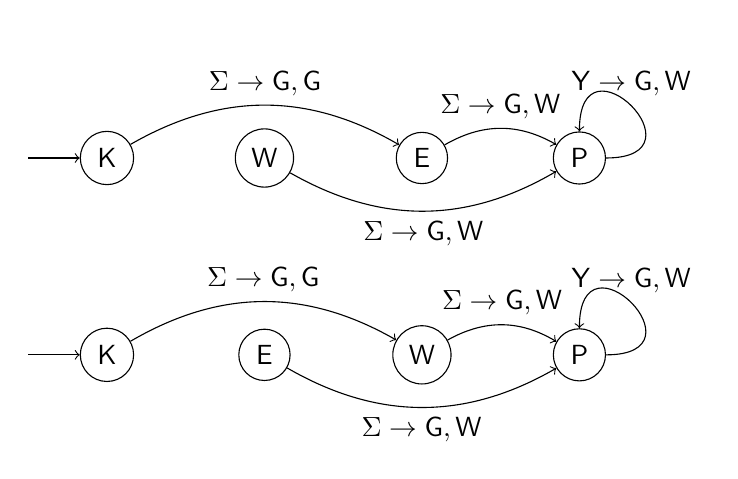
\begin{tikzpicture}
      \node[draw, circle] (P1) at (6, 0) {\sffamily P};
      \node[draw, circle] (W1) at (4, 0) {\sffamily W};
      \node[draw, circle] (E1) at (2, 0) {\sffamily E};
      \node[draw, circle] (K1) at (0, 0) {\sffamily K};
      \draw[->] (-1, 0) to (K1);
      \draw[->] (P1) to[in=90, out=0, looseness=7] node[midway, above] {$\q{Y} \rightarrow \q{G}, \q{W}$} (P1);
      \draw[->] (W1) to[bend left] node[midway, above] {$\Sigma \rightarrow \q{G}, \q{W}$} (P1);
      \draw[->] (E1) to[bend right] node[midway, below] {$\Sigma \rightarrow \q{G}, \q{W}$} (P1);
      \draw[->] (K1) to[bend left] node[midway, above] {$\Sigma \rightarrow \q{G}, \q{G}$} (W1);
      
      \node[draw, circle] (P2) at (6, 2.5) {\sffamily P};
      \node[draw, circle] (W2) at (2, 2.5) {\sffamily W};
      \node[draw, circle] (E2) at (4, 2.5) {\sffamily E};
      \node[draw, circle] (K2) at (0, 2.5) {\sffamily K};
      \draw[->] (-1, 2.5) to (K2);
      \draw[->] (P2) to[in=90, out=0, looseness=7] node[midway, above] {$\q{Y} \rightarrow \q{G}, \q{W}$} (P2);
      \draw[->] (W2) to[bend right] node[midway, below] {$\Sigma \rightarrow \q{G}, \q{W}$} (P2);
      \draw[->] (E2) to[bend left] node[midway, above] {$\Sigma \rightarrow \q{G}, \q{W}$} (P2);
      \draw[->] (K2) to[bend left] node[midway, above] {$\Sigma \rightarrow \q{G}, \q{G}$} (E2);
    \end{tikzpicture}
  \end{center}
  \caption{Two equivalent machines (\texttt{\#xAA00000} and \texttt{\#xCC00000}).}
  \label{fig:renaming-states}
\end{figure}

Two Turing machines $M_1$ and $M_2$ are identical if $M_2$
can be produced by renaming states in $M_1$. The Emu
and Wombat states may be swapped in a Platypus machine; but the
Kangaroo and Platypus states cannot be swapped with other states,
as the Kangaroo state is always the initial state, and the Platypus
state always is missing a transition.

A traversal of the machine can be used to normalise a mirror image,
mapping the first state other than Kangaroo or Platypus encountered
to the Emu state. I use a depth-first traversal, visiting the transition
on reading Yellow first, though the particular traversal used does not
affect efficacy. The traversal builds a new machine with the mapping
applied. However, it could be possible that both the Emu and Wombat
states are dead, so no assignment is possible; this algorithm does
not ever insert transitions from dead states, implicitly performing
dead-code elimination, and so the mapping does not matter.

54,494,608 unique machines (20.3\%) remain after renaming states.
This figure is very close to half the machines remaining after
dead code elimination, but 200 machines do not have live Emu or
Wombat states, and so cannot be normalised. The results are
presented in Figure~\ref{fig:rename}. The most apparent change is
that there are no machines which transition to Emu from
Kangaroo upon reading either colour; those machines have Emu
remapped to Wombat, as that transition is visited first.
It took 141 CPU-seconds to rename every Platypus machine.

\begin{figure}
  \begin{center}
    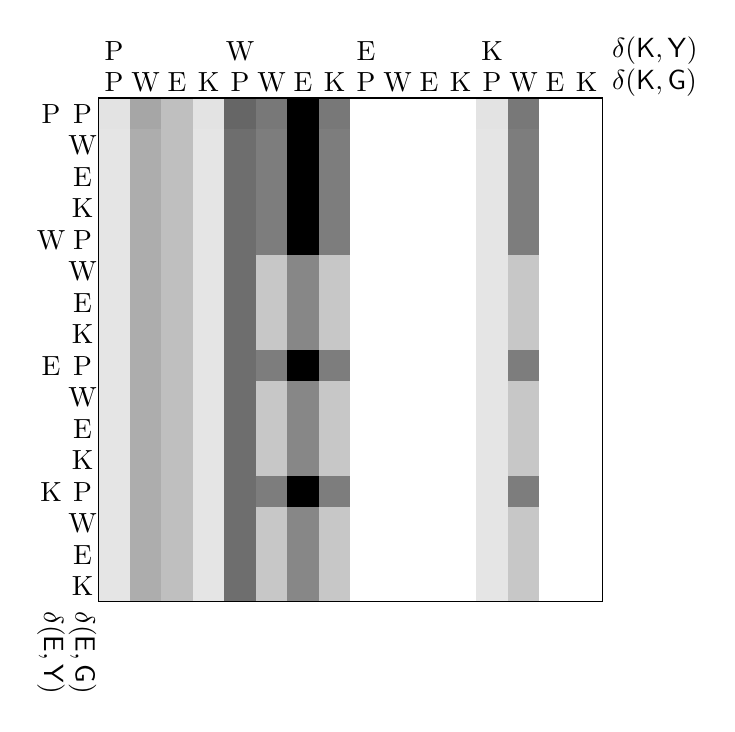
\begin{tikzpicture}[yscale=-1, scale=0.4]
  \node[anchor=west] at (16, -1.5) {$\delta (\q{K}, \q{Y})$};
  \node[anchor=west] at (16, -0.5) {$\delta (\q{K}, \q{G})$};
  \node[anchor=west, rotate=-90] at (-1.5, 16) {$\delta (\q{E}, \q{Y})$};
  \node[anchor=west, rotate=-90] at (-0.5, 16) {$\delta (\q{E}, \q{G})$};
  \node at (0.5, -1.5) {P}; \node at (-1.5, 0.5) {P};
  \node at (0.5, -0.5) {P}; \node at (-0.5, 0.5) {P};
  \node at (4.5, -0.5) {P}; \node at (-0.5, 4.5) {P};
  \node at (8.5, -0.5) {P}; \node at (-0.5, 8.5) {P};
  \node at (12.5, -0.5) {P}; \node at (-0.5, 12.5) {P};
  \node at (4.5, -1.5) {W}; \node at (-1.5, 4.5) {W};
  \node at (1.5, -0.5) {W}; \node at (-0.5, 1.5) {W};
  \node at (5.5, -0.5) {W}; \node at (-0.5, 5.5) {W};
  \node at (9.5, -0.5) {W}; \node at (-0.5, 9.5) {W};
  \node at (13.5, -0.5) {W}; \node at (-0.5, 13.5) {W};
  \node at (8.5, -1.5) {E}; \node at (-1.5, 8.5) {E};
  \node at (2.5, -0.5) {E}; \node at (-0.5, 2.5) {E};
  \node at (6.5, -0.5) {E}; \node at (-0.5, 6.5) {E};
  \node at (10.5, -0.5) {E}; \node at (-0.5, 10.5) {E};
  \node at (14.5, -0.5) {E}; \node at (-0.5, 14.5) {E};
  \node at (12.5, -1.5) {K}; \node at (-1.5, 12.5) {K};
  \node at (3.5, -0.5) {K}; \node at (-0.5, 3.5) {K};
  \node at (7.5, -0.5) {K}; \node at (-0.5, 7.5) {K};
  \node at (11.5, -0.5) {K}; \node at (-0.5, 11.5) {K};
  \node at (15.5, -0.5) {K}; \node at (-0.5, 15.5) {K};
  \fill[black!11!white] (0, 0) rectangle +(1, 1);
  \fill[black!10!white] (0, 1) rectangle +(1, 1);
  \fill[black!10!white] (0, 2) rectangle +(1, 1);
  \fill[black!10!white] (0, 3) rectangle +(1, 1);
  \fill[black!10!white] (0, 4) rectangle +(1, 1);
  \fill[black!10!white] (0, 5) rectangle +(1, 1);
  \fill[black!10!white] (0, 6) rectangle +(1, 1);
  \fill[black!10!white] (0, 7) rectangle +(1, 1);
  \fill[black!10!white] (0, 8) rectangle +(1, 1);
  \fill[black!10!white] (0, 9) rectangle +(1, 1);
  \fill[black!10!white] (0, 10) rectangle +(1, 1);
  \fill[black!10!white] (0, 11) rectangle +(1, 1);
  \fill[black!10!white] (0, 12) rectangle +(1, 1);
  \fill[black!10!white] (0, 13) rectangle +(1, 1);
  \fill[black!10!white] (0, 14) rectangle +(1, 1);
  \fill[black!10!white] (0, 15) rectangle +(1, 1);
  \fill[black!35!white] (1, 0) rectangle +(1, 1);
  \fill[black!32!white] (1, 1) rectangle +(1, 1);
  \fill[black!32!white] (1, 2) rectangle +(1, 1);
  \fill[black!32!white] (1, 3) rectangle +(1, 1);
  \fill[black!32!white] (1, 4) rectangle +(1, 1);
  \fill[black!32!white] (1, 5) rectangle +(1, 1);
  \fill[black!32!white] (1, 6) rectangle +(1, 1);
  \fill[black!32!white] (1, 7) rectangle +(1, 1);
  \fill[black!32!white] (1, 8) rectangle +(1, 1);
  \fill[black!32!white] (1, 9) rectangle +(1, 1);
  \fill[black!32!white] (1, 10) rectangle +(1, 1);
  \fill[black!32!white] (1, 11) rectangle +(1, 1);
  \fill[black!32!white] (1, 12) rectangle +(1, 1);
  \fill[black!32!white] (1, 13) rectangle +(1, 1);
  \fill[black!32!white] (1, 14) rectangle +(1, 1);
  \fill[black!32!white] (1, 15) rectangle +(1, 1);
  \fill[black!25!white] (2, 0) rectangle +(1, 1);
  \fill[black!25!white] (2, 1) rectangle +(1, 1);
  \fill[black!25!white] (2, 2) rectangle +(1, 1);
  \fill[black!25!white] (2, 3) rectangle +(1, 1);
  \fill[black!25!white] (2, 4) rectangle +(1, 1);
  \fill[black!25!white] (2, 5) rectangle +(1, 1);
  \fill[black!25!white] (2, 6) rectangle +(1, 1);
  \fill[black!25!white] (2, 7) rectangle +(1, 1);
  \fill[black!25!white] (2, 8) rectangle +(1, 1);
  \fill[black!25!white] (2, 9) rectangle +(1, 1);
  \fill[black!25!white] (2, 10) rectangle +(1, 1);
  \fill[black!25!white] (2, 11) rectangle +(1, 1);
  \fill[black!25!white] (2, 12) rectangle +(1, 1);
  \fill[black!25!white] (2, 13) rectangle +(1, 1);
  \fill[black!25!white] (2, 14) rectangle +(1, 1);
  \fill[black!25!white] (2, 15) rectangle +(1, 1);
  \fill[black!11!white] (3, 0) rectangle +(1, 1);
  \fill[black!10!white] (3, 1) rectangle +(1, 1);
  \fill[black!10!white] (3, 2) rectangle +(1, 1);
  \fill[black!10!white] (3, 3) rectangle +(1, 1);
  \fill[black!10!white] (3, 4) rectangle +(1, 1);
  \fill[black!10!white] (3, 5) rectangle +(1, 1);
  \fill[black!10!white] (3, 6) rectangle +(1, 1);
  \fill[black!10!white] (3, 7) rectangle +(1, 1);
  \fill[black!10!white] (3, 8) rectangle +(1, 1);
  \fill[black!10!white] (3, 9) rectangle +(1, 1);
  \fill[black!10!white] (3, 10) rectangle +(1, 1);
  \fill[black!10!white] (3, 11) rectangle +(1, 1);
  \fill[black!10!white] (3, 12) rectangle +(1, 1);
  \fill[black!10!white] (3, 13) rectangle +(1, 1);
  \fill[black!10!white] (3, 14) rectangle +(1, 1);
  \fill[black!10!white] (3, 15) rectangle +(1, 1);
  \fill[black!60!white] (4, 0) rectangle +(1, 1);
  \fill[black!57!white] (4, 1) rectangle +(1, 1);
  \fill[black!57!white] (4, 2) rectangle +(1, 1);
  \fill[black!57!white] (4, 3) rectangle +(1, 1);
  \fill[black!57!white] (4, 4) rectangle +(1, 1);
  \fill[black!57!white] (4, 5) rectangle +(1, 1);
  \fill[black!57!white] (4, 6) rectangle +(1, 1);
  \fill[black!57!white] (4, 7) rectangle +(1, 1);
  \fill[black!57!white] (4, 8) rectangle +(1, 1);
  \fill[black!57!white] (4, 9) rectangle +(1, 1);
  \fill[black!57!white] (4, 10) rectangle +(1, 1);
  \fill[black!57!white] (4, 11) rectangle +(1, 1);
  \fill[black!57!white] (4, 12) rectangle +(1, 1);
  \fill[black!57!white] (4, 13) rectangle +(1, 1);
  \fill[black!57!white] (4, 14) rectangle +(1, 1);
  \fill[black!57!white] (4, 15) rectangle +(1, 1);
  \fill[black!53!white] (5, 0) rectangle +(1, 1);
  \fill[black!51!white] (5, 1) rectangle +(1, 1);
  \fill[black!51!white] (5, 2) rectangle +(1, 1);
  \fill[black!51!white] (5, 3) rectangle +(1, 1);
  \fill[black!51!white] (5, 4) rectangle +(1, 1);
  \fill[black!22!white] (5, 5) rectangle +(1, 1);
  \fill[black!22!white] (5, 6) rectangle +(1, 1);
  \fill[black!22!white] (5, 7) rectangle +(1, 1);
  \fill[black!51!white] (5, 8) rectangle +(1, 1);
  \fill[black!22!white] (5, 9) rectangle +(1, 1);
  \fill[black!22!white] (5, 10) rectangle +(1, 1);
  \fill[black!22!white] (5, 11) rectangle +(1, 1);
  \fill[black!51!white] (5, 12) rectangle +(1, 1);
  \fill[black!22!white] (5, 13) rectangle +(1, 1);
  \fill[black!22!white] (5, 14) rectangle +(1, 1);
  \fill[black!22!white] (5, 15) rectangle +(1, 1);
  \fill[black!100!white] (6, 0) rectangle +(1, 1);
  \fill[black!100!white] (6, 1) rectangle +(1, 1);
  \fill[black!100!white] (6, 2) rectangle +(1, 1);
  \fill[black!100!white] (6, 3) rectangle +(1, 1);
  \fill[black!100!white] (6, 4) rectangle +(1, 1);
  \fill[black!47!white] (6, 5) rectangle +(1, 1);
  \fill[black!47!white] (6, 6) rectangle +(1, 1);
  \fill[black!47!white] (6, 7) rectangle +(1, 1);
  \fill[black!100!white] (6, 8) rectangle +(1, 1);
  \fill[black!47!white] (6, 9) rectangle +(1, 1);
  \fill[black!47!white] (6, 10) rectangle +(1, 1);
  \fill[black!47!white] (6, 11) rectangle +(1, 1);
  \fill[black!100!white] (6, 12) rectangle +(1, 1);
  \fill[black!47!white] (6, 13) rectangle +(1, 1);
  \fill[black!47!white] (6, 14) rectangle +(1, 1);
  \fill[black!47!white] (6, 15) rectangle +(1, 1);
  \fill[black!53!white] (7, 0) rectangle +(1, 1);
  \fill[black!51!white] (7, 1) rectangle +(1, 1);
  \fill[black!51!white] (7, 2) rectangle +(1, 1);
  \fill[black!51!white] (7, 3) rectangle +(1, 1);
  \fill[black!51!white] (7, 4) rectangle +(1, 1);
  \fill[black!22!white] (7, 5) rectangle +(1, 1);
  \fill[black!22!white] (7, 6) rectangle +(1, 1);
  \fill[black!22!white] (7, 7) rectangle +(1, 1);
  \fill[black!51!white] (7, 8) rectangle +(1, 1);
  \fill[black!22!white] (7, 9) rectangle +(1, 1);
  \fill[black!22!white] (7, 10) rectangle +(1, 1);
  \fill[black!22!white] (7, 11) rectangle +(1, 1);
  \fill[black!51!white] (7, 12) rectangle +(1, 1);
  \fill[black!22!white] (7, 13) rectangle +(1, 1);
  \fill[black!22!white] (7, 14) rectangle +(1, 1);
  \fill[black!22!white] (7, 15) rectangle +(1, 1);
  \fill[black!0!white] (8, 0) rectangle +(1, 1);
  \fill[black!0!white] (8, 1) rectangle +(1, 1);
  \fill[black!0!white] (8, 2) rectangle +(1, 1);
  \fill[black!0!white] (8, 3) rectangle +(1, 1);
  \fill[black!0!white] (8, 4) rectangle +(1, 1);
  \fill[black!0!white] (8, 5) rectangle +(1, 1);
  \fill[black!0!white] (8, 6) rectangle +(1, 1);
  \fill[black!0!white] (8, 7) rectangle +(1, 1);
  \fill[black!0!white] (8, 8) rectangle +(1, 1);
  \fill[black!0!white] (8, 9) rectangle +(1, 1);
  \fill[black!0!white] (8, 10) rectangle +(1, 1);
  \fill[black!0!white] (8, 11) rectangle +(1, 1);
  \fill[black!0!white] (8, 12) rectangle +(1, 1);
  \fill[black!0!white] (8, 13) rectangle +(1, 1);
  \fill[black!0!white] (8, 14) rectangle +(1, 1);
  \fill[black!0!white] (8, 15) rectangle +(1, 1);
  \fill[black!0!white] (9, 0) rectangle +(1, 1);
  \fill[black!0!white] (9, 1) rectangle +(1, 1);
  \fill[black!0!white] (9, 2) rectangle +(1, 1);
  \fill[black!0!white] (9, 3) rectangle +(1, 1);
  \fill[black!0!white] (9, 4) rectangle +(1, 1);
  \fill[black!0!white] (9, 5) rectangle +(1, 1);
  \fill[black!0!white] (9, 6) rectangle +(1, 1);
  \fill[black!0!white] (9, 7) rectangle +(1, 1);
  \fill[black!0!white] (9, 8) rectangle +(1, 1);
  \fill[black!0!white] (9, 9) rectangle +(1, 1);
  \fill[black!0!white] (9, 10) rectangle +(1, 1);
  \fill[black!0!white] (9, 11) rectangle +(1, 1);
  \fill[black!0!white] (9, 12) rectangle +(1, 1);
  \fill[black!0!white] (9, 13) rectangle +(1, 1);
  \fill[black!0!white] (9, 14) rectangle +(1, 1);
  \fill[black!0!white] (9, 15) rectangle +(1, 1);
  \fill[black!0!white] (10, 0) rectangle +(1, 1);
  \fill[black!0!white] (10, 1) rectangle +(1, 1);
  \fill[black!0!white] (10, 2) rectangle +(1, 1);
  \fill[black!0!white] (10, 3) rectangle +(1, 1);
  \fill[black!0!white] (10, 4) rectangle +(1, 1);
  \fill[black!0!white] (10, 5) rectangle +(1, 1);
  \fill[black!0!white] (10, 6) rectangle +(1, 1);
  \fill[black!0!white] (10, 7) rectangle +(1, 1);
  \fill[black!0!white] (10, 8) rectangle +(1, 1);
  \fill[black!0!white] (10, 9) rectangle +(1, 1);
  \fill[black!0!white] (10, 10) rectangle +(1, 1);
  \fill[black!0!white] (10, 11) rectangle +(1, 1);
  \fill[black!0!white] (10, 12) rectangle +(1, 1);
  \fill[black!0!white] (10, 13) rectangle +(1, 1);
  \fill[black!0!white] (10, 14) rectangle +(1, 1);
  \fill[black!0!white] (10, 15) rectangle +(1, 1);
  \fill[black!0!white] (11, 0) rectangle +(1, 1);
  \fill[black!0!white] (11, 1) rectangle +(1, 1);
  \fill[black!0!white] (11, 2) rectangle +(1, 1);
  \fill[black!0!white] (11, 3) rectangle +(1, 1);
  \fill[black!0!white] (11, 4) rectangle +(1, 1);
  \fill[black!0!white] (11, 5) rectangle +(1, 1);
  \fill[black!0!white] (11, 6) rectangle +(1, 1);
  \fill[black!0!white] (11, 7) rectangle +(1, 1);
  \fill[black!0!white] (11, 8) rectangle +(1, 1);
  \fill[black!0!white] (11, 9) rectangle +(1, 1);
  \fill[black!0!white] (11, 10) rectangle +(1, 1);
  \fill[black!0!white] (11, 11) rectangle +(1, 1);
  \fill[black!0!white] (11, 12) rectangle +(1, 1);
  \fill[black!0!white] (11, 13) rectangle +(1, 1);
  \fill[black!0!white] (11, 14) rectangle +(1, 1);
  \fill[black!0!white] (11, 15) rectangle +(1, 1);
  \fill[black!11!white] (12, 0) rectangle +(1, 1);
  \fill[black!10!white] (12, 1) rectangle +(1, 1);
  \fill[black!10!white] (12, 2) rectangle +(1, 1);
  \fill[black!10!white] (12, 3) rectangle +(1, 1);
  \fill[black!10!white] (12, 4) rectangle +(1, 1);
  \fill[black!10!white] (12, 5) rectangle +(1, 1);
  \fill[black!10!white] (12, 6) rectangle +(1, 1);
  \fill[black!10!white] (12, 7) rectangle +(1, 1);
  \fill[black!10!white] (12, 8) rectangle +(1, 1);
  \fill[black!10!white] (12, 9) rectangle +(1, 1);
  \fill[black!10!white] (12, 10) rectangle +(1, 1);
  \fill[black!10!white] (12, 11) rectangle +(1, 1);
  \fill[black!10!white] (12, 12) rectangle +(1, 1);
  \fill[black!10!white] (12, 13) rectangle +(1, 1);
  \fill[black!10!white] (12, 14) rectangle +(1, 1);
  \fill[black!10!white] (12, 15) rectangle +(1, 1);
  \fill[black!53!white] (13, 0) rectangle +(1, 1);
  \fill[black!51!white] (13, 1) rectangle +(1, 1);
  \fill[black!51!white] (13, 2) rectangle +(1, 1);
  \fill[black!51!white] (13, 3) rectangle +(1, 1);
  \fill[black!51!white] (13, 4) rectangle +(1, 1);
  \fill[black!22!white] (13, 5) rectangle +(1, 1);
  \fill[black!22!white] (13, 6) rectangle +(1, 1);
  \fill[black!22!white] (13, 7) rectangle +(1, 1);
  \fill[black!51!white] (13, 8) rectangle +(1, 1);
  \fill[black!22!white] (13, 9) rectangle +(1, 1);
  \fill[black!22!white] (13, 10) rectangle +(1, 1);
  \fill[black!22!white] (13, 11) rectangle +(1, 1);
  \fill[black!51!white] (13, 12) rectangle +(1, 1);
  \fill[black!22!white] (13, 13) rectangle +(1, 1);
  \fill[black!22!white] (13, 14) rectangle +(1, 1);
  \fill[black!22!white] (13, 15) rectangle +(1, 1);
  \fill[black!0!white] (14, 0) rectangle +(1, 1);
  \fill[black!0!white] (14, 1) rectangle +(1, 1);
  \fill[black!0!white] (14, 2) rectangle +(1, 1);
  \fill[black!0!white] (14, 3) rectangle +(1, 1);
  \fill[black!0!white] (14, 4) rectangle +(1, 1);
  \fill[black!0!white] (14, 5) rectangle +(1, 1);
  \fill[black!0!white] (14, 6) rectangle +(1, 1);
  \fill[black!0!white] (14, 7) rectangle +(1, 1);
  \fill[black!0!white] (14, 8) rectangle +(1, 1);
  \fill[black!0!white] (14, 9) rectangle +(1, 1);
  \fill[black!0!white] (14, 10) rectangle +(1, 1);
  \fill[black!0!white] (14, 11) rectangle +(1, 1);
  \fill[black!0!white] (14, 12) rectangle +(1, 1);
  \fill[black!0!white] (14, 13) rectangle +(1, 1);
  \fill[black!0!white] (14, 14) rectangle +(1, 1);
  \fill[black!0!white] (14, 15) rectangle +(1, 1);
  \fill[black!0!white] (15, 0) rectangle +(1, 1);
  \fill[black!0!white] (15, 1) rectangle +(1, 1);
  \fill[black!0!white] (15, 2) rectangle +(1, 1);
  \fill[black!0!white] (15, 3) rectangle +(1, 1);
  \fill[black!0!white] (15, 4) rectangle +(1, 1);
  \fill[black!0!white] (15, 5) rectangle +(1, 1);
  \fill[black!0!white] (15, 6) rectangle +(1, 1);
  \fill[black!0!white] (15, 7) rectangle +(1, 1);
  \fill[black!0!white] (15, 8) rectangle +(1, 1);
  \fill[black!0!white] (15, 9) rectangle +(1, 1);
  \fill[black!0!white] (15, 10) rectangle +(1, 1);
  \fill[black!0!white] (15, 11) rectangle +(1, 1);
  \fill[black!0!white] (15, 12) rectangle +(1, 1);
  \fill[black!0!white] (15, 13) rectangle +(1, 1);
  \fill[black!0!white] (15, 14) rectangle +(1, 1);
  \fill[black!0!white] (15, 15) rectangle +(1, 1);
  \draw (0, 0) rectangle (16, 16);
\end{tikzpicture}
  \end{center}
  \caption{A heatmap of the distribution of unique machines after renaming states.}
  \label{fig:rename}
\end{figure}

\section{DFA minimisation}

One form of redundancy which dead code elimination cannot identify
is when two states have the same effects. Consider the
(part of a) machine in Figure~\ref{fig:equivalent-states} for example:
intuitively the machine always keeps the board unchanged, and
always moves towards the Ghost Gum tree. More formally, its two states
are equivalent, as outgoing transitions from the states have the same effects,
and the outgoing transitions target states which are equivalent, so
the states can be merged as in Figure~\ref{fig:normalised-states}. Dead
code elimination cannot normalise this machine further, as both states
are live. Renaming could only normalise the mirror image of the former
machine to the former machine.

\begin{figure}
  \begin{subfigure}[b]{0.5\textwidth}
    \begin{center}
      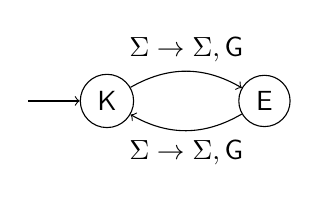
\begin{tikzpicture}
        \node[draw,circle](K) at (0, 0) {\sffamily K};
        \node[draw,circle](E) at (2, 0) {\sffamily E};
        \draw[->] (-1, 0) -- (K);
        \path[->] (K) edge[bend left]
        node[pos=0.5, above] {$\Sigma \rightarrow \Sigma, \q{G}$}
        (E);
        \path[->] (E) edge[bend left]
        node[pos=0.5, below] {$\Sigma \rightarrow \Sigma, \q{G}$}
        (K);
      \end{tikzpicture}
    \end{center}
    \caption{Before normalisation.}
    \label{fig:equivalent-states}
  \end{subfigure}
  \begin{subfigure}[b]{0.5\textwidth}
    \begin{center}
      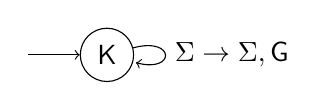
\begin{tikzpicture}
        \node[draw,circle](K) at (0, 0) {\sffamily K};
        \draw[->] (-1, 0) -- (K);
        \path[->] (K) edge[loop right]
        node[pos=0.5, right] {$\Sigma \rightarrow \Sigma, \q{G}$}
        (K);
      \end{tikzpicture}
    \end{center}
    \caption{After normalisation.}
    \label{fig:normalised-states}
  \end{subfigure}
  \caption{A machine with two equivalent states.}
\end{figure}

\subsection{Extending DFA minimisation}

An algorithm for minimising discrete finite automata (DFAs) can
identify a similar redundancy in DFAs. Baumann
\cite{baumann} extends Hopcroft's algorithm \cite{hopcroft} to identify
redundant states in \emph{Mealy~machines} \cite{mealy}, by requiring
that transitions must also produce the same outputs in order to be
equivalent. I treat Platypus machines as Mealy machines, with the
output of each transition being the direction to move and the colour
to write of the transition, i.e. the action on the board. This \emph{abstraction}
applied to a Turing machine is depicted in Figure~\ref{fig:mealy}.

\begin{figure}
  \begin{center}
    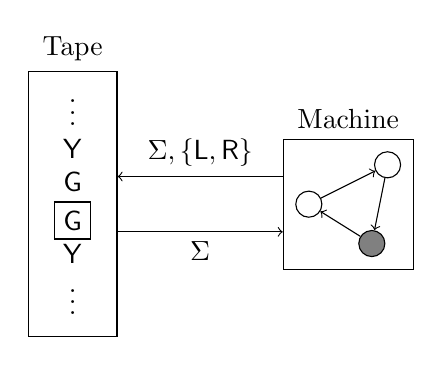
\begin{tikzpicture}
      % Mealy machine
      \node[draw,circle](A) at (0.0, 0.5) {};
      \node[draw,circle](B) at (1, 1) {};
      \node[fill,gray, circle](C) at (0.8, 0) {};
      \node[draw,circle] at (0.8, 0) {}; % outline for C
      \draw[->] (A) -- (B);
      \draw[->] (B) -- (C);
      \draw[->] (C) -- (A);
      \node[draw, fit=(A) (B) (C), inner sep=1ex] (Mealy) {};
      \node[above=0ex of Mealy] {Machine};

      \node[draw, inner sep=1ex](Tape) at (-3, 0.5) {
        $\begin{array}{c}
            \vdots \\ \q{Y} \\ \q{G} \\ \fbox{$\q{G}$} \\ \q{Y} \\ \vdots
         \end{array}$
      };
      \node[above=0ex of Tape] {Tape};
      \draw[transform canvas={yshift=1em}, ->] (Mealy) -- (Tape) node[pos=0.5, above] {$\Sigma, \{\q{L}, \q{R}\}$};
      \draw[transform canvas={yshift=-1em}, ->] (Tape) -- (Mealy) node[midway, below] {$\Sigma$};
    \end{tikzpicture}
  \end{center}
  
  \caption{A Turing machine may be abstracted as a Mealy machine.}
  \label{fig:mealy}
\end{figure}

This abstraction may seem odd, as a Turing machine is
more powerful than a Mealy machine. But a result of the abstraction
is that the minimisation algorithm only now does not model the state
of the tape at all, providing a conservative and sound approximation of
the Turing machine. The tape only ensures that that some particular
sequences of outputs may prevent the machine from receiving
some sequences of inputs; an equivalence algorithm for Mealy
machines is unaware of this constraint, and thus an equivalence
algorithm only considers execution paths which can never occur. For
example, if a Turing machine writes a symbol to a cell then immediately
reads the same cell, the machine can only read that symbol again; but an
equivalence algorithm will needlessly consider what would occur if the
machine reads any symbol. Thus the algorithm is conservative but safe --
it may unnecessarily split equivalence classes, but the abstraction will
not cause the algorithm to unsoundly merge equivalence classes.

But we cannot trust the state of a Platypus board when reasoning
about one Platypus machine anyway, as the opponent of a machine may
(more or less) arbitrarily modify the board, invalidating any assumptions
about the state of the board. For example, a machine which always fills
the board with Yellow is not distinguishable from a machine which
always preserves the state of the board, if only that one machine uses the board.
(Recall that the board is initially all Yellow.) Introducing another
machine which concurrently fills the board with Green provokes
different behaviour out of the Yellow-filling and board-preserving
machines, and so they are not equivalent.

Also note that states must be partitioned by the number of outgoing
transitions, as Platypus machines are incomplete by definition. Thus
the minimisation algorithm begins with the equivalence sets
$\setb{\setb{\q{Platypus}}, \setb{\q{Wombat}, \q{Emu}, \q{Kangaroo}}}$.

\subsection{Implementation}

I implemented a fast version of Nerode's algorithm for minimising
DFAs \cite{nerode}. Though the algorithm has worse complexity
($\mathcal{O}(n^2)$ for $n$ states) than Hopcroft's algorithm
($\mathcal{O}(n \log n)$) the number of states is small, allowing for
constant factors to have large influence on performance, and the
algorithm lends itself to data parallelism with a
\emph{single instruction-multiple data} (SIMD) implementation.

In essence the algorithm iteratively constructs an array containing
which denotes pairs of states which are distinguishable. Let $A$ be
this array, where $A_{a, b}$ denotes that the states $a$ and $b$ may
be distinguished. $A$ is symmetric, i.e.
$ \forall a, b\ldotp A_{a, b} = A_{b, a} $. Initially $A_{a, b}$ is set to
if $a$ and $b$ have a different number of outgoing
states, or the transitions leaving $a$ and $b$ have different effects.
Then the array is iterated by marking states as distinct when they
have transitions which lead to distinct states. The algorithm
terminates when no elements of $A$ are changed.
Each state $S$ is then renamed to the highest-numbered state that
is not distinct from $S$ according to $A$. This renaming notably
preserves the Platypus state, as no other states will ever be equivalent
to the Platypus state, and the algorithm preserves the Kangaroo state,
as it has the greatest index per the representation in Section~\ref{sec:representation}.

As forementioned the algorithm can be implemented with data parallelism.
The SIMD extensions for x86 beginning with the \emph{Streaming SIMD Extensions} (SSE)
offer operations which perform an operation on each of 16 byte-sized \emph{lanes}
at once, which allows the entirety of $A$ to be updated in parallel, if each
element is stored as one byte.\footnote{Note that $A$ is two-dimensional, but
  a vector is one-dimensional, so the implementation must convert
  two-dimensional indices to one-dimensional indices. I chose to use
  \emph{row-major order} to be consistent with arrays in Common Lisp, but
  this decision is arbitrary and does not affect the behaviour of the algorithm.}
The most difficult part of a SIMD implementation
is following transitions, which require two particular permutations of the lanes
to compute derivatives, and then an arbitrary permutation in order to index $A$
with the derivatives. Fortunately, there is an operation to perform an arbitrary
permutation, namely the \emph{shuffle} operation\footnote{Although the \texttt{pshufb}
  instruction was only introduced in the \emph{Supplemental Streaming SIMD
    Extensions 3} (SSSE3) instruction set. I envy the person who gets to come up with
  these names.};
its use follows the approach Geoff Langdale used for implementing discrete finite
automata with SIMD code \cite{sheng,hyperscan}. The algorithm is presented in
Figure~\ref{fig:nerode}, though for \emph{complete} Mealy machines to simplify
presentation. The algorithm must treat undefined transitions as distinct from
any defined transition in order to handle \emph{incomplete} machines; for
example, such treatment must be given for reading a Green cell from the Platypus
state with a Platypus machine.

\begin{figure}
  \begin{center}
    \begin{tabular}{l}
      \emph{Set up initial state and target lookup table} \\
      \textbf{for each state} a, b, \textbf{each symbol} s \\
      \quad distinct[states $\times$ a + b] $\leftarrow$ output(a, s) $\neq$ output(b, s) \\
      \textbf{for each state} q, \textbf{each symbol} s \\
      \quad target[symbols $\times$ q + s] = target(q, s) \\
      rows = row indices \\
      cols = column indices \\
      \emph{Row-major access functions} \\
      A(a, b) = shuffle(vector: distinct, indices: states $\times$ a + b) \\
      out(q, s) = shuffle(vector: target, indices: symbols $\times$ q + s) \\
      \emph{Iterate} \\
      \textbf{while} distinct \textbf{changes} \\
      \quad \textbf{for each symbol} s \\
      \quad\quad distinct $\leftarrow$ distinct $\lor$ A(target(rows, s), target(columns, s))
    \end{tabular}
  \end{center}
  \caption{Iterating Nerode's algorithm with SIMD code.}
  \label{fig:nerode}
\end{figure}

I have yet to analyse the complexity of the parallel algorithm, but its
\emph{depth} must be in $\mathcal{O}(n^2)$, as at worst the algorithm
can only avoid termination by updating two elements (due to symmetry)
of the $n^2$ elements of $A$ which was previously false.
In practice processing every Platypus machine requires very few
iterations; 227 million machines require just one iteration, 41 million
require two iterations, and 602 thousand require three.

The algorithm may be extended to larger machines
(such as busy beaver machines) when larger SIMD operations are
available. The AVX-512 extension provides instructions
which work in parallel over 64 bytes for example, allowing for the
minimisation of 8-state machines. The \emph{Neon} extension for
ARM includes a \texttt{tbl} instruction which can shuffle from a 64
byte table, despite Neon only providing 16 byte operations otherwise;
the other operations would have to be performed four times.

107,452,240 unique machines (40.03\%) remain after minimisation.
This is only barely better than dead code elimination, and much
worse than renaming, as minimisation cannot detect mirror images.
Performing renaming after minimisation yields a similarly slight
improvement with 53,726,320 unique machines (20.01\%) remaining. The
results of the combined algorithms are not visually distinguishable from
the results of renaming alone, though it eliminates 83.1 trillion matches
from the Platypus tournament due to the quadratic time complexity of
the tournament. It took 359 CPU-seconds to perform minimisation and
renaming of all Platypus machines.

\section{Differential testing}

I have argued that the proposed algorithms are sound, but bugs may still arise
in the implementation of these algorithms. The implementations of the
algorithms are concise: DCE and renaming are implemented each with
less than 30 lines of code, and DFA minimisation consists of 52 lines of code%
\footnote{This figure does not include the 40 lines of code used to manipulate
  the representation of Platypus machines. The functions manipulating the
  representation are trivial, performing no mutation and minimal
  control flow, and may be tested independently, so I am less concerned about
  bugs in the representation.}, so it is feasible to manually inspect the
implementations. I used \emph{differential testing} to try to find cases where
normalisation does not produce an equivalent machine to be safe. The testing
program generates two random machines and asserts that normalisation
does not change the outcome of a match between the machines, i.e.

$$\forall m, n\ldotp \q{run}(m, n) = \q{run}(\q{normalise}(m), n) = \q{run}(m, \q{normalise}(n))$$

The testing program initially detected a bug in the Platypus game interpreter,
which managed to incorrectly decode a machine, leading to deviations
between a machine and normalisation of the machine. Dead code elimination
and renaming were tested for 30 billion games each, without finding any errors.
The testing program was also instrumental in finding several bugs in the
implementation of DFA minimisation.

\section{Heuristics}

It may be the case that few equivalence sets cover most of the machines,
and so approximate results can be found by running just those
equivalence sets. Figure~\ref{fig:coverage} shows the coverage produced by
combined DFA minimisation and renaming; a mere 1\% of the equivalence
sets cover over 55\% of the machines, but coverage only increases linearly
past a few percent. Almost all equivalence sets only contain two machines,
as every machine has a mirror image. While the coverage of so few equivalence
sets is interesting, it is still too small to produce useful approximations in
my opinion.

\begin{figure}
  \centering
  \begin{tikzpicture}
    \begin{axis}[
      xlabel=Proportion of sets covered,
      ylabel=Proportion of machines covered,
      width=0.8\textwidth, height=8cm]
      \addplot[mark=none] table[x=amount, y=density, col sep=comma] {early-stopping.csv};
    \end{axis}
  \end{tikzpicture}
  \caption{The machines covered by testing varying amounts of equivalence sets.}
  \label{fig:coverage}
\end{figure}

\chapter{Running a tournament}

\section{Interpreters}

The remaining games after detecting equivalences must be played
quickly to be able to get a result in an acceptable time frame.
I implemented two \emph{interpreters} for Platypus matches, one which
uses scalar code and one which uses SIMD code. Both may be parallelised
over multiple cores. The interpreters are implemented in the file
\texttt{Code/run-game.lisp}.

The interpreters play a member of each \emph{equivalence set} produced
by equivalence detection, rather than playing every possible player
against another. Thus the points and win achieved from a match must
be weighted by the size of the equivalence set of the opponent, as one
such match is being performed in place of a match for each member
of the opposing equivalence set. For example, if Player 1 scores $10$ points
against a Player 2 chosen from an equivalence set of $2^{20}$ machines,
$10 \times 2^{20}$ points must be added to the total score of Player 1.

\subsection{Naïve interpreter}

The na\"ive interpreter runs one match on each core. The board is also
represented as an integer (with each bit representing a cell of the board)
to avoid accessing memory.

\subsection{SIMD interpreter}

The SIMD interpreter runs eight matches at once, one in each 32-bit lane
of the 256-bit operands used in operations in the \emph{Advanced Vector
  Extensions 2} (AVX2) instruction set. The interpreter works by playing
all games with one player set to the same player, and the other player
being read from the array of players. The wins and points accumulated
by games are counted in each lane. Running each match is relatively
simple, as all data used by the Platypus game can fit into 32-bit lanes,
and AVX2 provides all of the operations needed to run a Platypus game.

One issue with running a tournament in a SIMD manner is that
games vary in how long they take to complete: some finish after just
a few turns, and some run the full 50 turns. A simple use of SIMD would
be to run a game in each lane, and wait until all games finish. But
waiting for all games in all lanes to finish could thus be inefficient,
if a longer game in one lane prevents the other lanes from being
\emph{refilled}. Such a situation with 8 games played using 4 lanes is
depicted in Figure~\ref{fig:refill-all-policy}. Another simple use would be
to wait until some number of games finish and then use scalar code to
refill each lane, but the scalar code can easily become a bottleneck.

\newcommand{\game}[4]{
  \draw[fill=white] (#1, #2) rectangle +(#3, 0.5);
  \node at (#1 + 0.25, #2 + 0.25) {#4};
}
\begin{figure}
  \begin{subfigure}[b]{\textwidth}
    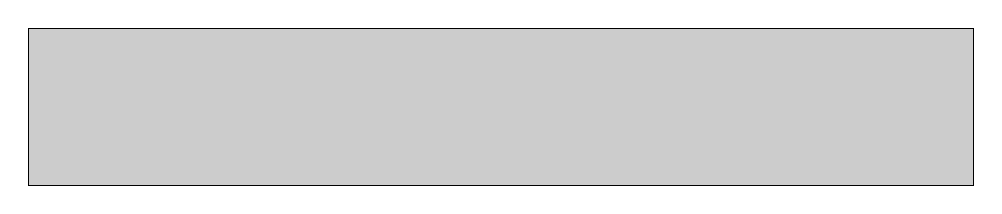
\begin{tikzpicture}
      \draw[fill=black!20!white] (0, 0) rectangle (12, 2);
      \game{0}{1.5}{1}{1}
      \game{0}{1}{1}{2}
      \game{0}{0.5}{6}{3}
      \game{0}{0}{1}{4}
      \game{6}{1.5}{6}{5}
      \game{6}{1}{1}{6}
      \game{6}{0.5}{1}{7}
      \game{6}{0}{1}{8}
    \end{tikzpicture}
    \caption{Refill when all games have finished.}
    \label{fig:refill-all-policy}
  \end{subfigure}
  
  \vspace{1em}
  
  \begin{subfigure}[b]{\textwidth}
    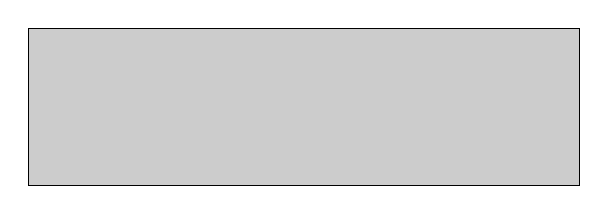
\begin{tikzpicture}
      \draw[fill=black!20!white] (0, 0) rectangle (7, 2);
      \game{0}{1.5}{1}{1}
      \game{0}{1}{1}{2}
      \game{0}{0.5}{6}{3}
      \game{0}{0}{1}{4}
      \game{1}{1.5}{6}{5}
      \game{1}{1}{1}{6}
      \game{6}{0.5}{1}{7}
      \game{1}{0}{1}{8}
    \end{tikzpicture}
    \caption{Refill when any game has finished.}
    \label{fig:refill-any-policy}
  \end{subfigure}
  \caption{How work is performed by different policies on when to refill.}
\end{figure}

Instead I manage and refill each lane individually. The SIMD interpreter
refills all lanes before taking a turn, by loading a vector of machines from
the array starting at a \emph{cursor} position, then \emph{expanding}%
\footnote{The name \emph{expand} comes from APL \cite{expand-apl}.
  Expand is implemented as an instruction in AVX-512, but AVX2
  lacks an expand instruction; so I use a lookup table to determine
  the right shuffle to do (in \texttt{+expand-table+} in \texttt{Code/vector.lisp}).}
new machines into the lanes which have finished games, and incrementing the
cursor by the number of lanes that were refilled. The tricky part of this
operation is depicted in Figure~\ref{fig:refill-algorithm}. The interpreter also
accumulates the points which the constant player acquired and
if the constant player won into counters for each lane; the 50 turns for
all $2^{28}$ machines conveniently could not possibly overflow a 32-bit
counter. Refilling each lane individually produces a work distribution
like Figure~\ref{fig:refill-any-policy}. The remaining machines are processed by
the na\"ive interpreter when there are too few remaining machines to fit into
a full\footnote{A full vector must be loaded before expansion, regardless of how
  many lanes actually get refilled.} vector. This policy provides $1.32\times$ the
throughput of refilling when all lanes are finished with 12 threads, and
$1.15\times$ the throughput with 24 threads.

\begin{figure}
  \begin{center}
    \begin{tabular}{|l|c|c|c|c|}
      \hline
      players  & 1 & 2 & 3 & 4 \\
      finished & F & T & T & F \\
      new-players & 5 & 6 & 7 & 8 \\
      \hline
      expanded := \textsc{Expand}(values: new-players, mask: finished) & \dontcare & 5 & 6 & \dontcare \\
      \textsc{Select}(mask: finished, true: expanded, false: players) & 1 & 5 & 6 & 4 \\
      \hline
    \end{tabular}
  \end{center}
  
  \caption{A state of an interpreter which needs to be refilled,
    and the SIMD operations involved in refilling the state.
    (Values we don't care about are written as \dontcare{}.)}
  \label{fig:refill-algorithm}
\end{figure}

Differential testing was again useful while implementing the SIMD
interpreter: testing should always find that the results of running games
on the na\"ive interpreter and the SIMD interpreter are be identical. In
practise testing found bugs in transitioning from SIMD code to scalar code.

\subsection{GPGPU interpreter}

A graphics processing unit (GPU) also implements a SIMD paradigm, though
typically with more lanes following the same control flow. While a GPU is
usually used to render graphics as suggested by the name, \emph{general
  purpose computing on graphics processing units} (GPGPU) interfaces like
OpenCL and CUDA allow for performing a wider range of computations on
a GPU.

I implemented the SIMD interpreter in OpenCL, though I used a more na\"ive
refilling algorithm: the program assigns small chunks of the array of
machines to lanes, and has the OpenCL implementation assign chunks to
lanes.

\section{Aggregating results}

We must aggregate the results of games from each thread somehow. Such
aggregation is complicated by a game involving two machines, and that
we need to tally the results of both machines.

One approach is to have one global table of the results of all games played
thus far. However, updating this global table requires three atomic
increments. Another approach is that each thread could instead have its
own table, and tables are only summed together when the tournament is
finished, but this arrangement would require an exorbitant amount of
space with many cores.

Another is to avoid almost all global and atomic communication by
running all games involving one machine at a time, and only update the
results pertaining to that machine. The update needn't be atomic as only
one thread will ever update the tallies for one machine. However, a thread
must play all games where a machine is used as \emph{either} player,
which ends up duplicating the work which must be performed. Guy Steele
mentions, however, that ``good parallel code often performs redundant
operations to reduce communication'' \cite{organizing-functional-code}, so
we should investigate the idea nonetheless.

A hybrid would be to partition the space of $n$ machines into disjoint
ranges, and the space of $n^2$ matches into \emph{tiles}.
Each tile consists of $(\frac{n}{t})^2$ matches for some stripe count $t$. Each
thread operates on one tile at a time, with a thread-local table of $\frac{n}{t}$
machines for either player. Updates to the global table are inherently batched
by tiling; a thread would likely have better performance by locking to update
the global table, possibly with a separate lock for each of the $t$ stripes.

I chose to use the approach which avoids all global communication.
The approach is conceptually simple, unlike the tiling approach. The approach
is also a natural fit for the SIMD interpreter, which can only easily
record results for the constant player at a time: the results for the
other player would likely to be recorded out of order, as lanes may
be refilled at any time; for example, game \#3 finishes after games \#4, \#6
and \#8 despite starting first in Figure~\ref{fig:refill-any-policy}. It is possible to
\emph{scatter} the results into a local tile in the correct locations; but this
operation is slow in practice, and scatter instructions were only introduced
in the AVX-512 instruction set extension which none of my hardware supports.

Avoiding communication is also a good fit for processors which have
many cores and relatively slow communication between cores, unlike
the global table approach. For example, the 5900X processor has a worst-case
\emph{core-to-core latency} of 84 nanoseconds
\cite{core-to-core}, which is comparable to the average time it takes to
run a Platypus match; a larger processor such as the EPYC 7773X with
64 cores has a worst-case latency of 140 nanoseconds, and the worst-case
latency of a dual-processor system may exceed 200 nanoseconds
\cite{core-to-core-2}. It would be faster to duplicate work than to pay the cost
of communication with such high latency.

It appears that atomics are also slow on the GPU; performing atomic updates
after every match was about $2.3\times$ slower than only performing updates
after completing a chunk, and thus duplicating work to avoid communication
would be faster on the GPU. However, it is possible to \emph{scatter} with good
performance on a GPU, which would permit using the tiling approach. 

\section{Benchmarks}

The benchmark measures the maximum throughput achievable by a particular
configuration of thread count and interpreter. In particular, the benchmark
must be designed to simulate the ample work provided by the full Platypus
tournament, avoiding the effects of running out of work which might be caused
by issuing a fixed amount of work. Instead my benchmark keeps all threads
running for at least a minute, and measures how long it took between starting
the benchmark and the last results being submitted, which captures the
configuration running at full throughput.

I measured the power used by each configuration using a power meter.
My desktop computer draws around 90 watts while idle with only a graphical
session and Emacs running. The results are presented in Figure~\ref{fig:benchmarks}.

\begin{figure}
  \begin{center}
    \begin{tabular}{|r r|S[table-format=4.1,mode=text] r r r|}
      \hline
      Kind & Threads & {Throughput} & Days required & Power draw & Energy required\\
           & & {(Mmatches/s)} & & (W) & (kWh) \\
      \hline
      Na\"ive & 12 & 72.6 & 947 & 184 & 4182 \\
      Na\"ive & 24 & 88.6 & 776 & 184 & 3445 \\
      SIMD & 12 & 376 & 183 & 185 & 812 \\
      SIMD & 24 & 436 & 154 & 180 & 683 \\
      GPGPU & & 1062 & 65 & 223 & 348 \\
      \hline
    \end{tabular}
  \end{center}
  \caption{The performance and energy usage of some configurations of Platypus interpreters.}
  \label{fig:benchmarks}
\end{figure}

The SIMD and GPGPU interpreters are both more energy-efficient and
faster. The SIMD interpreter does not draw more power than the na\"ive
interpreter, though intuitively performing more transitions at once
would draw more power. Guermouche and Orgerie \cite{vectorized}
examined the power draw and energy use of running various high
performance computing applications with different vector widths, and
found that the variation in power draw was dependent on the
application and the processors used; one cluster would draw 28\%
more power using 256-bit vectors instead of 128-bit vectors, but one
computer would draw the same amount of power regardless of vector
width. However, they were able to use sensors in Intel processors to
more accurately determine the power draw of the processors and
memory independently; I used an external device which measures
the power draw of the whole computer.

\section{Distribution}
\label{sec:distribution}

Another option to utilise more hardware is to distribute the tournament
across multiple computers; running the tournament is embarrasingly
parallel as there are no dependencies between Platypus games. I distributed
the tournament by separating the tournament software into a \emph{server}
which allocates work and records results into a database, and a \emph{client}
which runs work on a GPU. The server is implemented in the
\texttt{Code/Distributed-host/} directory and the client is implemented
in the \texttt{Code/OpenCL-interpreter/} directory.

The tournament is run in two phases following the communication-avoiding
technique for aggregating results, with a phase for computing the results
of matches with a machine as either player.
The client communicates with the server by making HTTP requests. The client
first downloads the arrays of machines and equivalence set sizes to play.
The client then requests some machines to test, and the client plays those
machines against all opponent machines in the arrays. Multiple machines
are issued in one request to avoid network latency: with a tournament of the
53 million unique machines we found, a client which can play one billion
matches per second would otherwise need to make a request every 19
milliseconds. The client then submits the results to be stored in the database.

The distributed architecture happens to avoid gaps in the options which AWS
offers for GPU acceleration, though I was not trying to plan around the gaps.
A g5.xlarge instance offers one GPU, four virtual CPU cores and 16 GiB of
memory, but the next largest number of GPUs is provided with a g5.12xlarge
instance with 4 GPUs, 48 CPU cores and 192 GiB of memory. I do not need the
memory or CPUs, so it is more cost effective to use a larger number of
g5.xlarge instances.

Distribution also introduces some fault-tolerance. My prior experiences with
programming for GPGPU suggested that I could easily make mistakes while
manually managing CPU and GPU memory buffers; and assigning each GPU
to a separate process would isolate errors%
\footnote{Although it is difficult to \emph{detect} memory errors in the
  first place, so this is insufficient: memory-unsafe code will only crash
  if it accesses unmapped memory, and recently deallocated
  memory and off-by-one indices tend to still be mapped.}
and allow other client processes to continue running if one fails.

\section{Heuristics}

If many matches are short, an approximation of the full tournament
results can be found by stopping matches early. The lengths of one million
random matches are shown in Figure~\ref{fig:turn-distribution}; more than half
of all matches were shorter than 10 turns long, but again coverage past that point
is more gradual, except for the 170 thousand matches which hit the turn limit.
Note also the periodic nature of the distribution: there are local maxima at 2, 12,
22 and 31 turns, possibly related to machines taking 10 turns to wrap around the
board and reach each other again.

\begin{figure}
  \begin{subfigure}[b]{0.5\textwidth}
    \centering
    \begin{tikzpicture}
      \begin{axis}[
        xlabel=Turns,
        xmin=-1, xmax=51,
        ymin=0,
        ylabel=Matches,
        width=\textwidth, height=6cm, bar width=1]
        \addplot[ybar, fill=black] table[x=turns, y=count, col sep=comma] {match-lengths.csv};
      \end{axis}
    \end{tikzpicture}
  \end{subfigure}%
  \begin{subfigure}[b]{0.5\textwidth}
    \centering
    \begin{tikzpicture}
      \begin{axis}[
        xlabel=Maximum turns,
        xmin=-1, xmax=51,
        ymin=0,
        ylabel=Matches,
        width=\textwidth, height=6cm, bar width=1]
        \addplot[mark=none] table[x=turns, y=cumulative, col sep=comma] {match-lengths.csv};
      \end{axis}
    \end{tikzpicture}
  \end{subfigure}
  \caption{The distribution of the lengths of one million random matches.}
  \label{fig:turn-distribution}
\end{figure}

Many matches take all 50 turns; if such matches do not terminate
then cutting early may still pick the machine which would win a game
with the full length. The points scored by either machine could also be
extrapolated by scaling the numbers of points, assuming that the rate
at which points are scored remains constant throughout the game.
\chapter{Results}
\label{chap:results}

I ran the Platypus tournament using the facilities provided by
RMIT AWS Cloud Supercomputing (RACE), with the GPGPU
interpreter running all matches between equivalence sets
computed by the combined DFA minimisation and renaming
algorithm. It took about 17 GPU-days over 9 days to run the full
Platypus tournament using two g5.xlarge instances, with a
throughput of 3.7 billion Platypus matches per second.

I also analysed the best first and second players separately,
as the two-phase design described in \autoref{sec:distribution}
allows for recording the results separately.

\section{The full tournament}

A machine is involved in 536,870,912 matches (involving the
machine being either player against $2^{28}$ machines), and a
machine could win up to 26,843,545,600 points would it get the
maximum of 50 points in every game.

Tied for first place with 504,480,184 wins and 15,025,578,654 points are 32 machines equivalent to machine \texttt{2BEDC50}:

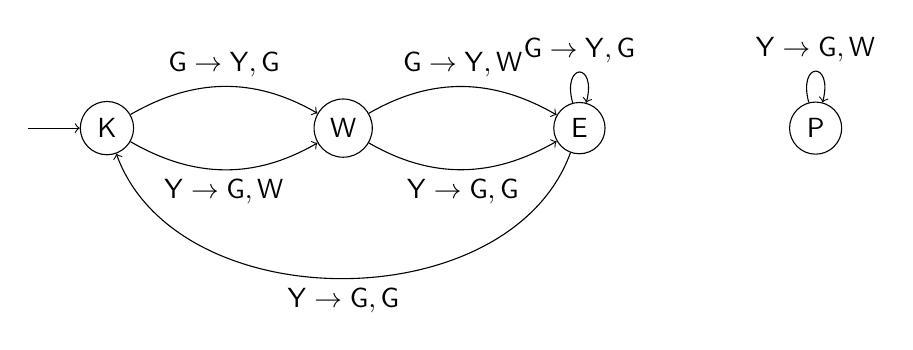
\begin{tikzpicture}
\node[draw, circle] (K) at (0, 0) {\sffamily K};
\node[draw, circle] (W) at (3, 0) {\sffamily W};
\node[draw, circle] (E) at (6, 0) {\sffamily E};
\node[draw, circle] (P) at (9, 0) {\sffamily P};
\draw[->] (-1, 0) to (K);
\draw[->] (K) to[out=-30, in=-150] node[midway, below] {$\q{Y} \rightarrow \q{G}, \q{W}$} (W);
\draw[->] (K) to[out=30, in=150] node[midway, above] {$\q{G} \rightarrow \q{Y}, \q{G}$} (W);
\draw[->] (E) to[out=-110, in=-70] node[midway, below] {$\q{Y} \rightarrow \q{G}, \q{G}$} (K);
\draw[->] (E) to[loop above] node[midway, above] {$\q{G} \rightarrow \q{Y}, \q{G}$} (E);
\draw[->] (W) to[out=-30, in=-150] node[midway, below] {$\q{Y} \rightarrow \q{G}, \q{G}$} (E);
\draw[->] (W) to[out=30, in=150] node[midway, above] {$\q{G} \rightarrow \q{Y}, \q{W}$} (E);
\draw[->] (P) to[loop above] node[midway, above] {$\q{Y} \rightarrow \q{G}, \q{W}$} (P);
\end{tikzpicture}

\noindent and 32 machines equivalent to machine \texttt{A3654D0}:

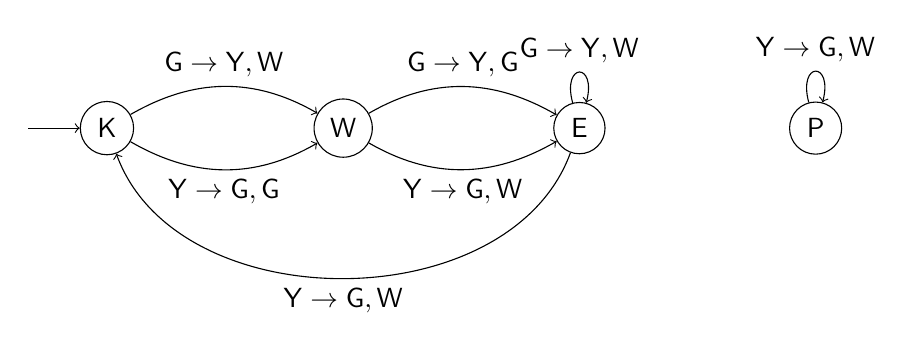
\begin{tikzpicture}
\node[draw, circle] (K) at (0, 0) {\sffamily K};
\node[draw, circle] (W) at (3, 0) {\sffamily W};
\node[draw, circle] (E) at (6, 0) {\sffamily E};
\node[draw, circle] (P) at (9, 0) {\sffamily P};
\draw[->] (-1, 0) to (K);
\draw[->] (K) to[out=-30, in=-150] node[midway, below] {$\q{Y} \rightarrow \q{G}, \q{G}$} (W);
\draw[->] (K) to[out=30, in=150] node[midway, above] {$\q{G} \rightarrow \q{Y}, \q{W}$} (W);
\draw[->] (E) to[out=-110, in=-70] node[midway, below] {$\q{Y} \rightarrow \q{G}, \q{W}$} (K);
\draw[->] (E) to[loop above] node[midway, above] {$\q{G} \rightarrow \q{Y}, \q{W}$} (E);
\draw[->] (W) to[out=-30, in=-150] node[midway, below] {$\q{Y} \rightarrow \q{G}, \q{W}$} (E);
\draw[->] (W) to[out=30, in=150] node[midway, above] {$\q{G} \rightarrow \q{Y}, \q{G}$} (E);
\draw[->] (P) to[loop above] node[midway, above] {$\q{Y} \rightarrow \q{G}, \q{W}$} (P);
\end{tikzpicture}

Tied for third place with 504,454,852 wins and 15,088,237,340 points are 32 machines equivalent to machine \texttt{2DE34F0}:

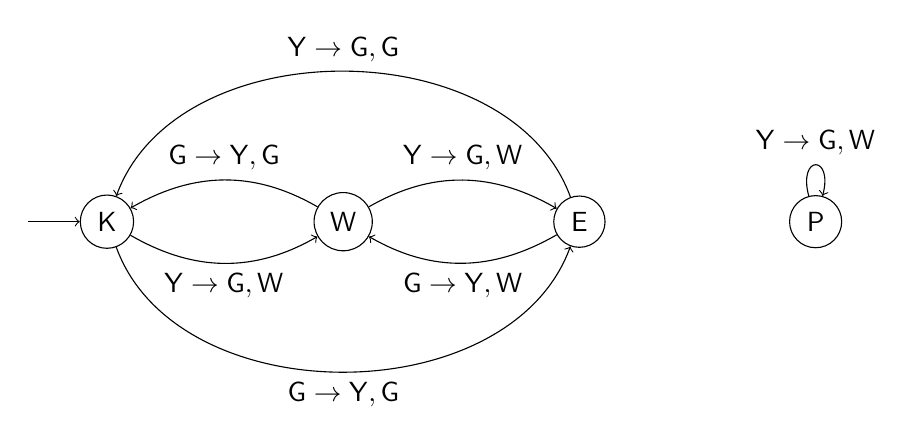
\begin{tikzpicture}
\node[draw, circle] (K) at (0, 0) {\sffamily K};
\node[draw, circle] (W) at (3, 0) {\sffamily W};
\node[draw, circle] (E) at (6, 0) {\sffamily E};
\node[draw, circle] (P) at (9, 0) {\sffamily P};
\draw[->] (-1, 0) to (K);
\draw[->] (K) to[out=-30, in=-150] node[midway, below] {$\q{Y} \rightarrow \q{G}, \q{W}$} (W);
\draw[->] (K) to[out=-70, in=-110] node[midway, below] {$\q{G} \rightarrow \q{Y}, \q{G}$} (E);
\draw[->] (E) to[out=110, in=70] node[midway, above] {$\q{Y} \rightarrow \q{G}, \q{G}$} (K);
\draw[->] (E) to[out=-150, in=-30] node[midway, below] {$\q{G} \rightarrow \q{Y}, \q{W}$} (W);
\draw[->] (W) to[out=30, in=150] node[midway, above] {$\q{Y} \rightarrow \q{G}, \q{W}$} (E);
\draw[->] (W) to[out=150, in=30] node[midway, above] {$\q{G} \rightarrow \q{Y}, \q{G}$} (K);
\draw[->] (P) to[loop above] node[midway, above] {$\q{Y} \rightarrow \q{G}, \q{W}$} (P);
\end{tikzpicture}

\noindent and 32 machines equivalent to machine \texttt{A56BC70}:

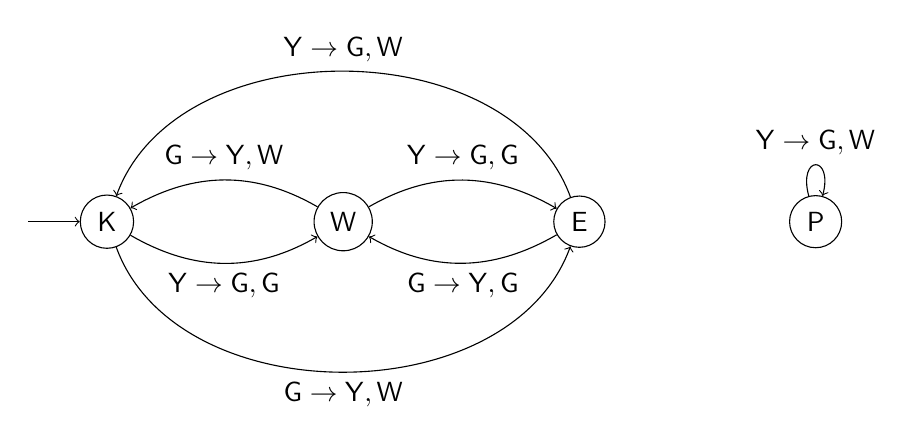
\begin{tikzpicture}
\node[draw, circle] (K) at (0, 0) {\sffamily K};
\node[draw, circle] (W) at (3, 0) {\sffamily W};
\node[draw, circle] (E) at (6, 0) {\sffamily E};
\node[draw, circle] (P) at (9, 0) {\sffamily P};
\draw[->] (-1, 0) to (K);
\draw[->] (K) to[out=-30, in=-150] node[midway, below] {$\q{Y} \rightarrow \q{G}, \q{G}$} (W);
\draw[->] (K) to[out=-70, in=-110] node[midway, below] {$\q{G} \rightarrow \q{Y}, \q{W}$} (E);
\draw[->] (E) to[out=110, in=70] node[midway, above] {$\q{Y} \rightarrow \q{G}, \q{W}$} (K);
\draw[->] (E) to[out=-150, in=-30] node[midway, below] {$\q{G} \rightarrow \q{Y}, \q{G}$} (W);
\draw[->] (W) to[out=30, in=150] node[midway, above] {$\q{Y} \rightarrow \q{G}, \q{G}$} (E);
\draw[->] (W) to[out=150, in=30] node[midway, above] {$\q{G} \rightarrow \q{Y}, \q{W}$} (K);
\draw[->] (P) to[loop above] node[midway, above] {$\q{Y} \rightarrow \q{G}, \q{W}$} (P);
\end{tikzpicture}

Tied for fifth place with 504,388,246 wins and 15,152,181,364 points are 32 machines equivalent to machine \texttt{AB634D0}:

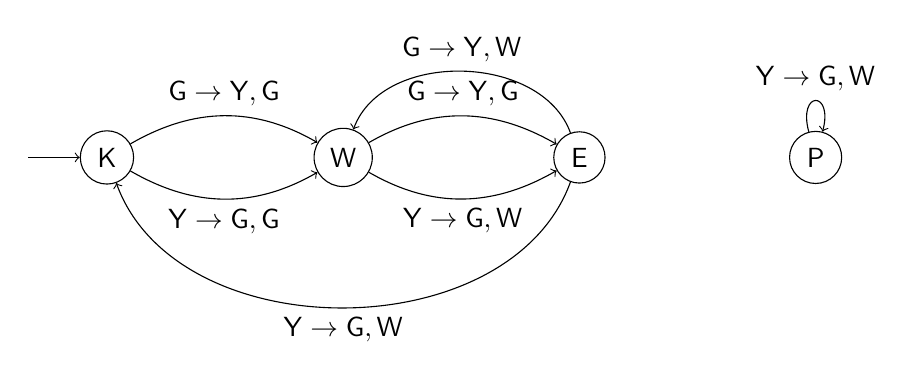
\begin{tikzpicture}
\node[draw, circle] (K) at (0, 0) {\sffamily K};
\node[draw, circle] (W) at (3, 0) {\sffamily W};
\node[draw, circle] (E) at (6, 0) {\sffamily E};
\node[draw, circle] (P) at (9, 0) {\sffamily P};
\draw[->] (-1, 0) to (K);
\draw[->] (K) to[out=-30, in=-150] node[midway, below] {$\q{Y} \rightarrow \q{G}, \q{G}$} (W);
\draw[->] (K) to[out=30, in=150] node[midway, above] {$\q{G} \rightarrow \q{Y}, \q{G}$} (W);
\draw[->] (E) to[out=-110, in=-70] node[midway, below] {$\q{Y} \rightarrow \q{G}, \q{W}$} (K);
\draw[->] (E) to[out=110, in=70] node[midway, above] {$\q{G} \rightarrow \q{Y}, \q{W}$} (W);
\draw[->] (W) to[out=-30, in=-150] node[midway, below] {$\q{Y} \rightarrow \q{G}, \q{W}$} (E);
\draw[->] (W) to[out=30, in=150] node[midway, above] {$\q{G} \rightarrow \q{Y}, \q{G}$} (E);
\draw[->] (P) to[loop above] node[midway, above] {$\q{Y} \rightarrow \q{G}, \q{W}$} (P);
\end{tikzpicture}

\noindent and 32 machines equivalent to machine \texttt{23EBC50}:

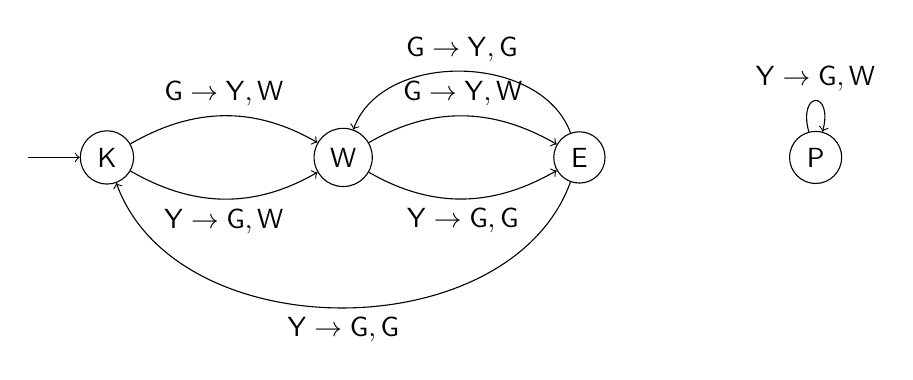
\begin{tikzpicture}
\node[draw, circle] (K) at (0, 0) {\sffamily K};
\node[draw, circle] (W) at (3, 0) {\sffamily W};
\node[draw, circle] (E) at (6, 0) {\sffamily E};
\node[draw, circle] (P) at (9, 0) {\sffamily P};
\draw[->] (-1, 0) to (K);
\draw[->] (K) to[out=-30, in=-150] node[midway, below] {$\q{Y} \rightarrow \q{G}, \q{W}$} (W);
\draw[->] (K) to[out=30, in=150] node[midway, above] {$\q{G} \rightarrow \q{Y}, \q{W}$} (W);
\draw[->] (E) to[out=-110, in=-70] node[midway, below] {$\q{Y} \rightarrow \q{G}, \q{G}$} (K);
\draw[->] (E) to[out=110, in=70] node[midway, above] {$\q{G} \rightarrow \q{Y}, \q{G}$} (W);
\draw[->] (W) to[out=-30, in=-150] node[midway, below] {$\q{Y} \rightarrow \q{G}, \q{G}$} (E);
\draw[->] (W) to[out=30, in=150] node[midway, above] {$\q{G} \rightarrow \q{Y}, \q{W}$} (E);
\draw[->] (P) to[loop above] node[midway, above] {$\q{Y} \rightarrow \q{G}, \q{W}$} (P);
\end{tikzpicture}

Tied for seventh place with 504,120,538 wins and 15,272,577,672 points are 32 machines equivalent to machine \texttt{23C74D0}:

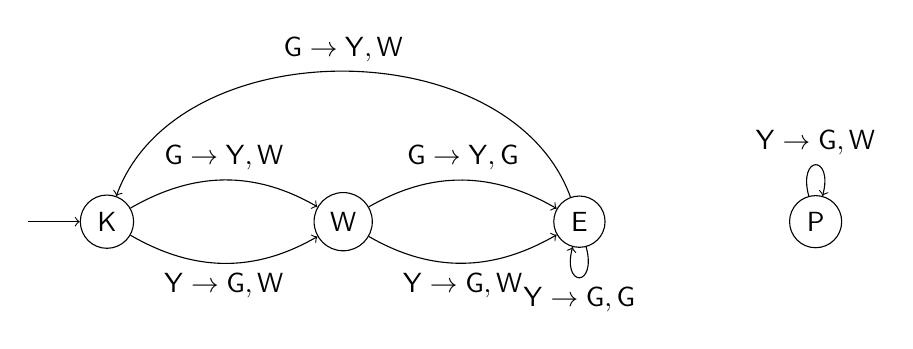
\begin{tikzpicture}
\node[draw, circle] (K) at (0, 0) {\sffamily K};
\node[draw, circle] (W) at (3, 0) {\sffamily W};
\node[draw, circle] (E) at (6, 0) {\sffamily E};
\node[draw, circle] (P) at (9, 0) {\sffamily P};
\draw[->] (-1, 0) to (K);
\draw[->] (K) to[out=-30, in=-150] node[midway, below] {$\q{Y} \rightarrow \q{G}, \q{W}$} (W);
\draw[->] (K) to[out=30, in=150] node[midway, above] {$\q{G} \rightarrow \q{Y}, \q{W}$} (W);
\draw[->] (E) to[loop below] node[midway, below] {$\q{Y} \rightarrow \q{G}, \q{G}$} (E);
\draw[->] (E) to[out=110, in=70] node[midway, above] {$\q{G} \rightarrow \q{Y}, \q{W}$} (K);
\draw[->] (W) to[out=-30, in=-150] node[midway, below] {$\q{Y} \rightarrow \q{G}, \q{W}$} (E);
\draw[->] (W) to[out=30, in=150] node[midway, above] {$\q{G} \rightarrow \q{Y}, \q{G}$} (E);
\draw[->] (P) to[loop above] node[midway, above] {$\q{Y} \rightarrow \q{G}, \q{W}$} (P);
\end{tikzpicture}

\noindent and 32 machines equivalent to machine \texttt{AB4FC50}:

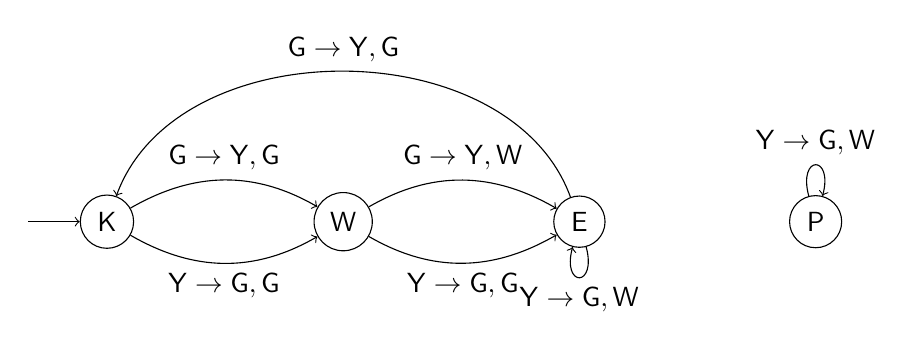
\begin{tikzpicture}
\node[draw, circle] (K) at (0, 0) {\sffamily K};
\node[draw, circle] (W) at (3, 0) {\sffamily W};
\node[draw, circle] (E) at (6, 0) {\sffamily E};
\node[draw, circle] (P) at (9, 0) {\sffamily P};
\draw[->] (-1, 0) to (K);
\draw[->] (K) to[out=-30, in=-150] node[midway, below] {$\q{Y} \rightarrow \q{G}, \q{G}$} (W);
\draw[->] (K) to[out=30, in=150] node[midway, above] {$\q{G} \rightarrow \q{Y}, \q{G}$} (W);
\draw[->] (E) to[loop below] node[midway, below] {$\q{Y} \rightarrow \q{G}, \q{W}$} (E);
\draw[->] (E) to[out=110, in=70] node[midway, above] {$\q{G} \rightarrow \q{Y}, \q{G}$} (K);
\draw[->] (W) to[out=-30, in=-150] node[midway, below] {$\q{Y} \rightarrow \q{G}, \q{G}$} (E);
\draw[->] (W) to[out=30, in=150] node[midway, above] {$\q{G} \rightarrow \q{Y}, \q{W}$} (E);
\draw[->] (P) to[loop above] node[midway, above] {$\q{Y} \rightarrow \q{G}, \q{W}$} (P);
\end{tikzpicture}

Tied for ninth place with 504,115,038 wins and 14,981,424,366 points are 32 machines equivalent to machine \texttt{2DE34B0}:

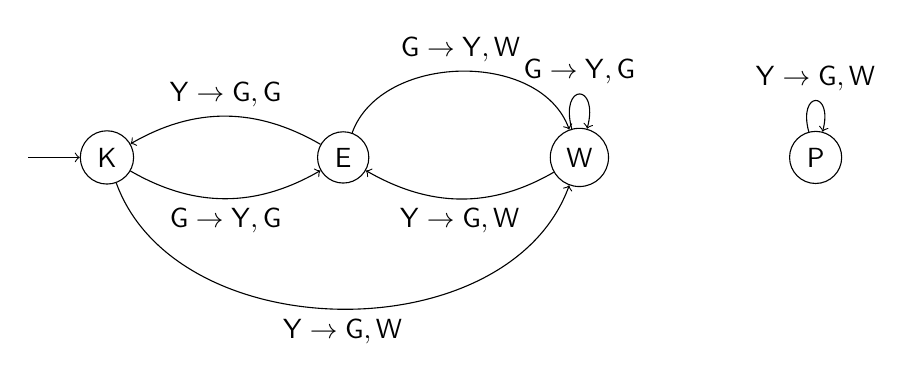
\begin{tikzpicture}
\node[draw, circle] (K) at (0, 0) {\sffamily K};
\node[draw, circle] (E) at (3, 0) {\sffamily E};
\node[draw, circle] (W) at (6, 0) {\sffamily W};
\node[draw, circle] (P) at (9, 0) {\sffamily P};
\draw[->] (-1, 0) to (K);
\draw[->] (K) to[out=-70, in=-110] node[midway, below] {$\q{Y} \rightarrow \q{G}, \q{W}$} (W);
\draw[->] (K) to[out=-30, in=-150] node[midway, below] {$\q{G} \rightarrow \q{Y}, \q{G}$} (E);
\draw[->] (E) to[out=150, in=30] node[midway, above] {$\q{Y} \rightarrow \q{G}, \q{G}$} (K);
\draw[->] (E) to[out=70, in=110] node[midway, above] {$\q{G} \rightarrow \q{Y}, \q{W}$} (W);
\draw[->] (W) to[out=-150, in=-30] node[midway, below] {$\q{Y} \rightarrow \q{G}, \q{W}$} (E);
\draw[->] (W) to[loop above] node[midway, above] {$\q{G} \rightarrow \q{Y}, \q{G}$} (W);
\draw[->] (P) to[loop above] node[midway, above] {$\q{Y} \rightarrow \q{G}, \q{W}$} (P);
\end{tikzpicture}

\noindent and 32 machines equivalent to machine \texttt{A56BC30}:

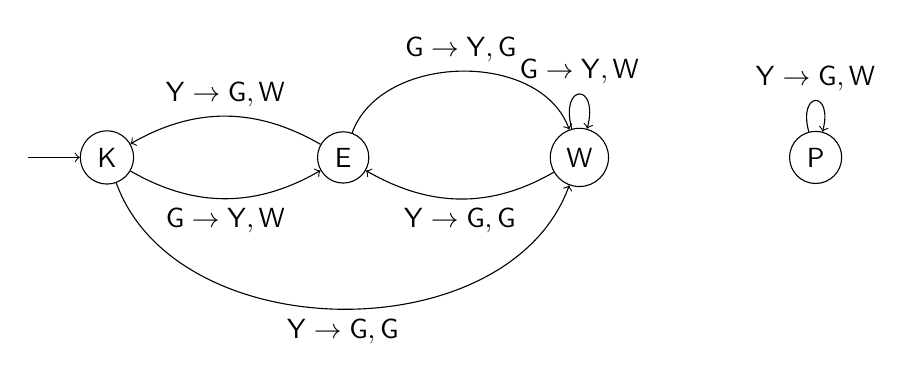
\begin{tikzpicture}
\node[draw, circle] (K) at (0, 0) {\sffamily K};
\node[draw, circle] (E) at (3, 0) {\sffamily E};
\node[draw, circle] (W) at (6, 0) {\sffamily W};
\node[draw, circle] (P) at (9, 0) {\sffamily P};
\draw[->] (-1, 0) to (K);
\draw[->] (K) to[out=-70, in=-110] node[midway, below] {$\q{Y} \rightarrow \q{G}, \q{G}$} (W);
\draw[->] (K) to[out=-30, in=-150] node[midway, below] {$\q{G} \rightarrow \q{Y}, \q{W}$} (E);
\draw[->] (E) to[out=150, in=30] node[midway, above] {$\q{Y} \rightarrow \q{G}, \q{W}$} (K);
\draw[->] (E) to[out=70, in=110] node[midway, above] {$\q{G} \rightarrow \q{Y}, \q{G}$} (W);
\draw[->] (W) to[out=-150, in=-30] node[midway, below] {$\q{Y} \rightarrow \q{G}, \q{G}$} (E);
\draw[->] (W) to[loop above] node[midway, above] {$\q{G} \rightarrow \q{Y}, \q{W}$} (W);
\draw[->] (P) to[loop above] node[midway, above] {$\q{Y} \rightarrow \q{G}, \q{W}$} (P);
\end{tikzpicture}

All of the transitions of the top ten equivalence sets always earn points
by changing the colour of tiles. None of the equivalence sets ever transition to
the Platypus state. The size of the equivalence sets is due to there being 16
configurations for the transition from Platypus upon reading a Yellow cell,
which is irrelevant as the Platypus state is unreachable, and 2 ways to assign
Emu and Wombat machines due to mirroring.

It is immediately evident that all positions in the top ten are ties between
two equivalence sets with similar structure. The only difference is that the
directions moved for every transition are flipped;
flipping the directions does not produce an equivalent machine, but flipping does
produce a machine which performs identically in a full tournament. A
match between machines $M_1$ and $M_2$ will have the same outcome as a
match between $M_1$ with directions flipped and $M_2$ with directions flipped.

\section{Player 1}

32 equivalence sets tied for first place as the first player, with
260,757,230 wins and 6,768,864,104 points. The equivalence sets include 2
machines equivalent to machine \texttt{3A34D2}:

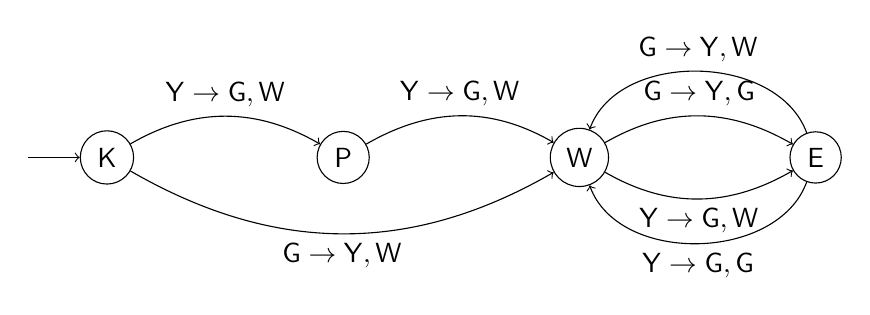
\begin{tikzpicture}
\node[draw, circle] (K) at (0, 0) {\sffamily K};
\node[draw, circle] (P) at (3, 0) {\sffamily P};
\node[draw, circle] (W) at (6, 0) {\sffamily W};
\node[draw, circle] (E) at (9, 0) {\sffamily E};
\draw[->] (-1, 0) to (K);
\draw[->] (K) to[out=30, in=150] node[midway, above] {$\q{Y} \rightarrow \q{G}, \q{W}$} (P);
\draw[->] (K) to[out=-30, in=-150] node[midway, below] {$\q{G} \rightarrow \q{Y}, \q{W}$} (W);
\draw[->] (E) to[out=-110, in=-70] node[midway, below] {$\q{Y} \rightarrow \q{G}, \q{G}$} (W);
\draw[->] (E) to[out=110, in=70] node[midway, above] {$\q{G} \rightarrow \q{Y}, \q{W}$} (W);
\draw[->] (W) to[out=-30, in=-150] node[midway, below] {$\q{Y} \rightarrow \q{G}, \q{W}$} (E);
\draw[->] (W) to[out=30, in=150] node[midway, above] {$\q{G} \rightarrow \q{Y}, \q{G}$} (E);
\draw[->] (P) to[out=30, in=150] node[midway, above] {$\q{Y} \rightarrow \q{G}, \q{W}$} (W);
\end{tikzpicture}

\noindent 2 machines equivalent to machine \texttt{8F2BC5A}:

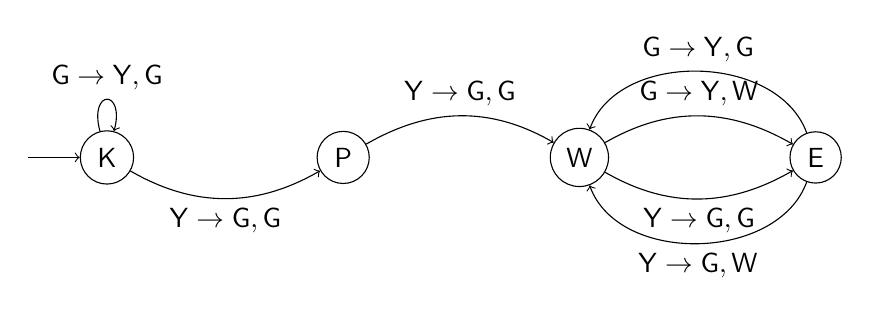
\begin{tikzpicture}
\node[draw, circle] (K) at (0, 0) {\sffamily K};
\node[draw, circle] (P) at (3, 0) {\sffamily P};
\node[draw, circle] (W) at (6, 0) {\sffamily W};
\node[draw, circle] (E) at (9, 0) {\sffamily E};
\draw[->] (-1, 0) to (K);
\draw[->] (K) to[out=-30, in=-150] node[midway, below] {$\q{Y} \rightarrow \q{G}, \q{G}$} (P);
\draw[->] (K) to[loop above] node[midway, above] {$\q{G} \rightarrow \q{Y}, \q{G}$} (K);
\draw[->] (E) to[out=-110, in=-70] node[midway, below] {$\q{Y} \rightarrow \q{G}, \q{W}$} (W);
\draw[->] (E) to[out=110, in=70] node[midway, above] {$\q{G} \rightarrow \q{Y}, \q{G}$} (W);
\draw[->] (W) to[out=-30, in=-150] node[midway, below] {$\q{Y} \rightarrow \q{G}, \q{G}$} (E);
\draw[->] (W) to[out=30, in=150] node[midway, above] {$\q{G} \rightarrow \q{Y}, \q{W}$} (E);
\draw[->] (P) to[out=30, in=150] node[midway, above] {$\q{Y} \rightarrow \q{G}, \q{G}$} (W);
\end{tikzpicture}

\noindent 2 machines equivalent to machine \texttt{05A34D2}:

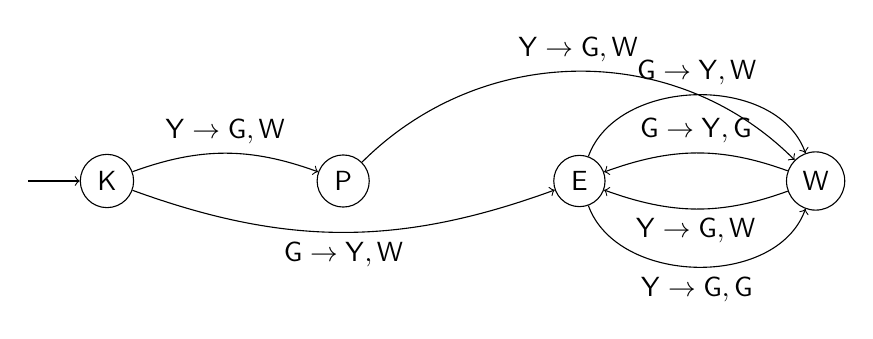
\begin{tikzpicture}
\node[draw, circle] (K) at (0, 0) {\sffamily K};
\node[draw, circle] (P) at (3, 0) {\sffamily P};
\node[draw, circle] (E) at (6, 0) {\sffamily E};
\node[draw, circle] (W) at (9, 0) {\sffamily W};
\draw[->] (-1, 0) to (K);
\draw[->] (K) to[out=-20, in=-160] node[midway, below] {$\q{G} \rightarrow \q{Y}, \q{W}$} (E);
\draw[->] (P) to[out=45, in=135] node[midway, above] {$\q{Y} \rightarrow \q{G}, \q{W}$} (W);
\draw[->] (K) to[out=20, in=160] node[midway, above] {$\q{Y} \rightarrow \q{G}, \q{W}$} (P);
\draw[->] (E) to[out=-70, in=-110] node[midway, below] {$\q{Y} \rightarrow \q{G}, \q{G}$} (W);
\draw[->] (E) to[out=70, in=110] node[midway, above] {$\q{G} \rightarrow \q{Y}, \q{W}$} (W);
\draw[->] (W) to[out=-160, in=-20] node[midway, below] {$\q{Y} \rightarrow \q{G}, \q{W}$} (E);
\draw[->] (W) to[out=160, in=20] node[midway, above] {$\q{G} \rightarrow \q{Y}, \q{G}$} (E);
\end{tikzpicture}

\noindent 2 machines equivalent to machine \texttt{822BC5A}:

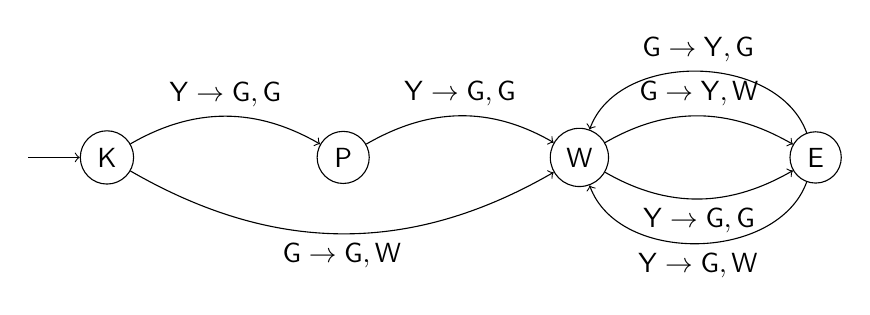
\begin{tikzpicture}
\node[draw, circle] (K) at (0, 0) {\sffamily K};
\node[draw, circle] (P) at (3, 0) {\sffamily P};
\node[draw, circle] (W) at (6, 0) {\sffamily W};
\node[draw, circle] (E) at (9, 0) {\sffamily E};
\draw[->] (-1, 0) to (K);
\draw[->] (K) to[out=30, in=150] node[midway, above] {$\q{Y} \rightarrow \q{G}, \q{G}$} (P);
\draw[->] (K) to[out=-30, in=-150] node[midway, below] {$\q{G} \rightarrow \q{G}, \q{W}$} (W);
\draw[->] (E) to[out=-110, in=-70] node[midway, below] {$\q{Y} \rightarrow \q{G}, \q{W}$} (W);
\draw[->] (E) to[out=110, in=70] node[midway, above] {$\q{G} \rightarrow \q{Y}, \q{G}$} (W);
\draw[->] (W) to[out=-30, in=-150] node[midway, below] {$\q{Y} \rightarrow \q{G}, \q{G}$} (E);
\draw[->] (W) to[out=30, in=150] node[midway, above] {$\q{G} \rightarrow \q{Y}, \q{W}$} (E);
\draw[->] (P) to[out=30, in=150] node[midway, above] {$\q{Y} \rightarrow \q{G}, \q{G}$} (W);
\end{tikzpicture}

\noindent and 2 machines equivalent to machine \texttt{0CA34D2}:

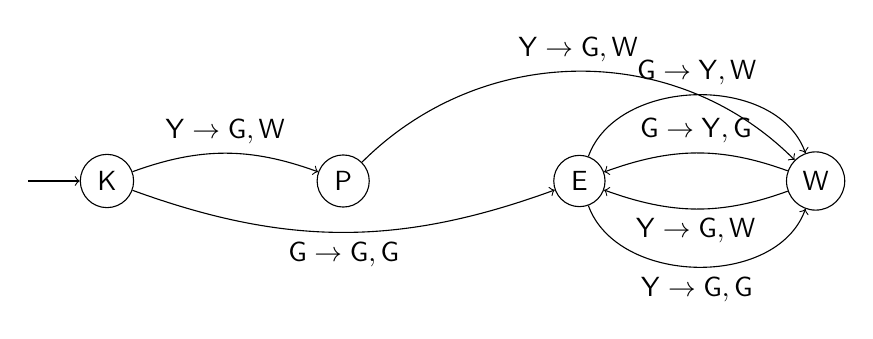
\begin{tikzpicture}
\node[draw, circle] (K) at (0, 0) {\sffamily K};
\node[draw, circle] (P) at (3, 0) {\sffamily P};
\node[draw, circle] (E) at (6, 0) {\sffamily E};
\node[draw, circle] (W) at (9, 0) {\sffamily W};
\draw[->] (-1, 0) to (K);
\draw[->] (K) to[out=-20, in=-160] node[midway, below] {$\q{G} \rightarrow \q{G}, \q{G}$} (E);
\draw[->] (P) to[out=45, in=135] node[midway, above] {$\q{Y} \rightarrow \q{G}, \q{W}$} (W);
\draw[->] (K) to[out=20, in=160] node[midway, above] {$\q{Y} \rightarrow \q{G}, \q{W}$} (P);
\draw[->] (E) to[out=-70, in=-110] node[midway, below] {$\q{Y} \rightarrow \q{G}, \q{G}$} (W);
\draw[->] (E) to[out=70, in=110] node[midway, above] {$\q{G} \rightarrow \q{Y}, \q{W}$} (W);
\draw[->] (W) to[out=-160, in=-20] node[midway, below] {$\q{Y} \rightarrow \q{G}, \q{W}$} (E);
\draw[->] (W) to[out=160, in=20] node[midway, above] {$\q{G} \rightarrow \q{Y}, \q{G}$} (E);
\end{tikzpicture}

Half of the redundancy can be explained by the forementioned flipping of directions,
leaving a 16-way tie. The only remaining difference between the machines is the
transition from the Kangaroo state upon reading a Green cell, which has 16 possible
configurations. The transition is never used as the first player always
reads yellow in its first turn, and none of the machines can reach the
Kangaroo state again. The Platypus state is however live in all of the top 32 equivalence
sets, but it also does not seem like the machines will halt the game because
a machine can only be in the Platypus state in its second turn, and there were not
enough turns before for the cell under the machine to be Green.

\section{Player 2}

Tied for first place with 244,410,400 wins and 8,048,411,604 points are 32 machines equivalent to machine \texttt{A56BC30}:

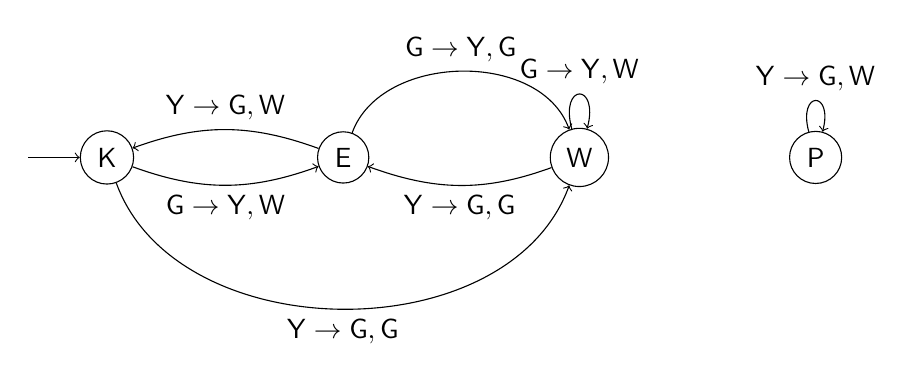
\begin{tikzpicture}
\node[draw, circle] (K) at (0, 0) {\sffamily K};
\node[draw, circle] (E) at (3, 0) {\sffamily E};
\node[draw, circle] (W) at (6, 0) {\sffamily W};
\node[draw, circle] (P) at (9, 0) {\sffamily P};
\draw[->] (-1, 0) to (K);
\draw[->] (K) to[out=-70, in=-110] node[midway, below] {$\q{Y} \rightarrow \q{G}, \q{G}$} (W);
\draw[->] (K) to[out=-20, in=-160] node[midway, below] {$\q{G} \rightarrow \q{Y}, \q{W}$} (E);
\draw[->] (E) to[out=160, in=20] node[midway, above] {$\q{Y} \rightarrow \q{G}, \q{W}$} (K);
\draw[->] (E) to[out=70, in=110] node[midway, above] {$\q{G} \rightarrow \q{Y}, \q{G}$} (W);
\draw[->] (W) to[out=-160, in=-20] node[midway, below] {$\q{Y} \rightarrow \q{G}, \q{G}$} (E);
\draw[->] (W) to[loop above] node[midway, above] {$\q{G} \rightarrow \q{Y}, \q{W}$} (W);
\draw[->] (P) to[loop above] node[midway, above] {$\q{Y} \rightarrow \q{G}, \q{W}$} (P);
\end{tikzpicture}

\noindent and 32 machines equivalent to machine \texttt{2DE34B0}:

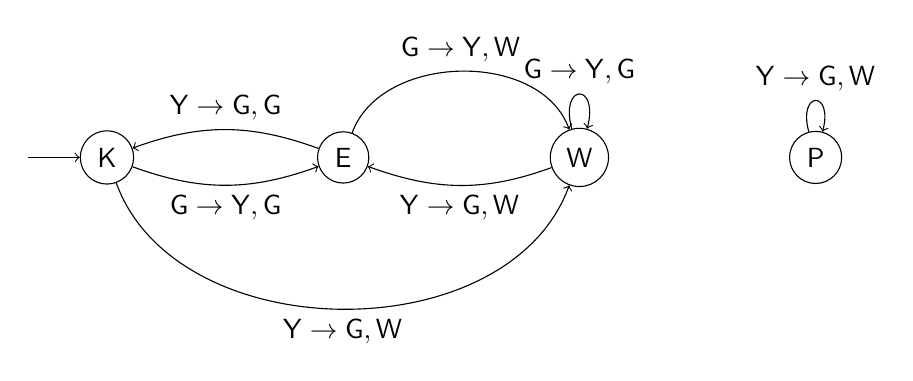
\begin{tikzpicture}
\node[draw, circle] (K) at (0, 0) {\sffamily K};
\node[draw, circle] (E) at (3, 0) {\sffamily E};
\node[draw, circle] (W) at (6, 0) {\sffamily W};
\node[draw, circle] (P) at (9, 0) {\sffamily P};
\draw[->] (-1, 0) to (K);
\draw[->] (K) to[out=-70, in=-110] node[midway, below] {$\q{Y} \rightarrow \q{G}, \q{W}$} (W);
\draw[->] (K) to[out=-20, in=-160] node[midway, below] {$\q{G} \rightarrow \q{Y}, \q{G}$} (E);
\draw[->] (E) to[out=160, in=20] node[midway, above] {$\q{Y} \rightarrow \q{G}, \q{G}$} (K);
\draw[->] (E) to[out=70, in=110] node[midway, above] {$\q{G} \rightarrow \q{Y}, \q{W}$} (W);
\draw[->] (W) to[out=-160, in=-20] node[midway, below] {$\q{Y} \rightarrow \q{G}, \q{W}$} (E);
\draw[->] (W) to[loop above] node[midway, above] {$\q{G} \rightarrow \q{Y}, \q{G}$} (W);
\draw[->] (P) to[loop above] node[midway, above] {$\q{Y} \rightarrow \q{G}, \q{W}$} (P);
\end{tikzpicture}

Tied for third place with 244,295,488 wins and 8,133,793,246 points are 32 machines equivalent to machine \texttt{23EBC50}:

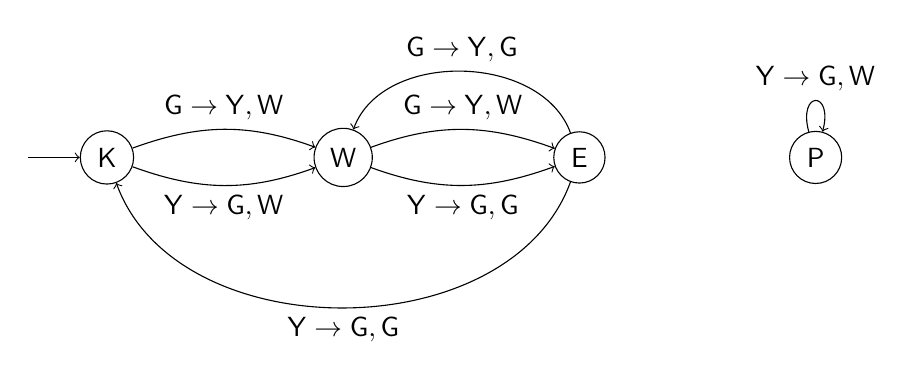
\begin{tikzpicture}
\node[draw, circle] (K) at (0, 0) {\sffamily K};
\node[draw, circle] (W) at (3, 0) {\sffamily W};
\node[draw, circle] (E) at (6, 0) {\sffamily E};
\node[draw, circle] (P) at (9, 0) {\sffamily P};
\draw[->] (-1, 0) to (K);
\draw[->] (E) to[out=-110, in=-70] node[midway, below] {$\q{Y} \rightarrow \q{G}, \q{G}$} (K);
\draw[->] (K) to[out=-20, in=-160] node[midway, below] {$\q{Y} \rightarrow \q{G}, \q{W}$} (W);
\draw[->] (K) to[out=20, in=160] node[midway, above] {$\q{G} \rightarrow \q{Y}, \q{W}$} (W);
\draw[->] (E) to[out=110, in=70] node[midway, above] {$\q{G} \rightarrow \q{Y}, \q{G}$} (W);
\draw[->] (W) to[out=-20, in=-160] node[midway, below] {$\q{Y} \rightarrow \q{G}, \q{G}$} (E);
\draw[->] (W) to[out=20, in=160] node[midway, above] {$\q{G} \rightarrow \q{Y}, \q{W}$} (E);
\draw[->] (P) to[loop above] node[midway, above] {$\q{Y} \rightarrow \q{G}, \q{W}$} (P);
\end{tikzpicture}

\noindent and 32 machines equivalent to machine \texttt{AB634D0}:

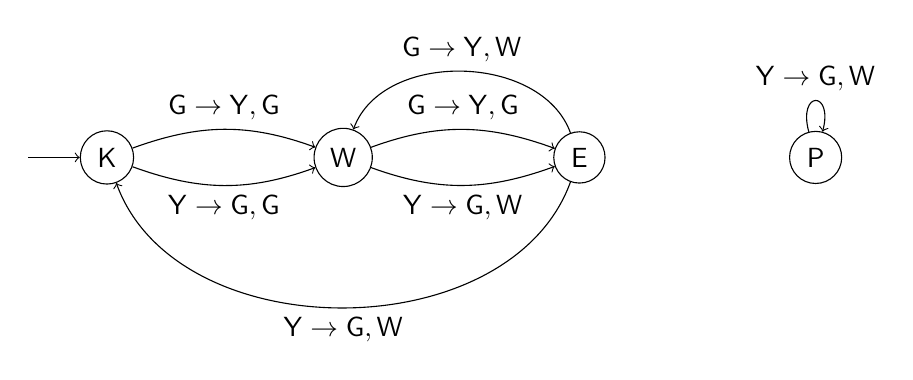
\begin{tikzpicture}
\node[draw, circle] (K) at (0, 0) {\sffamily K};
\node[draw, circle] (W) at (3, 0) {\sffamily W};
\node[draw, circle] (E) at (6, 0) {\sffamily E};
\node[draw, circle] (P) at (9, 0) {\sffamily P};
\draw[->] (-1, 0) to (K);
\draw[->] (E) to[out=-110, in=-70] node[midway, below] {$\q{Y} \rightarrow \q{G}, \q{W}$} (K);
\draw[->] (K) to[out=-20, in=-160] node[midway, below] {$\q{Y} \rightarrow \q{G}, \q{G}$} (W);
\draw[->] (K) to[out=20, in=160] node[midway, above] {$\q{G} \rightarrow \q{Y}, \q{G}$} (W);
\draw[->] (E) to[out=110, in=70] node[midway, above] {$\q{G} \rightarrow \q{Y}, \q{W}$} (W);
\draw[->] (W) to[out=-20, in=-160] node[midway, below] {$\q{Y} \rightarrow \q{G}, \q{W}$} (E);
\draw[->] (W) to[out=20, in=160] node[midway, above] {$\q{G} \rightarrow \q{Y}, \q{G}$} (E);
\draw[->] (P) to[loop above] node[midway, above] {$\q{Y} \rightarrow \q{G}, \q{W}$} (P);
\end{tikzpicture}

In fifth place with 244,268,960 wins and 8,240,095,104 points, 32 machines equivalent to machine \texttt{2BEDE50}:

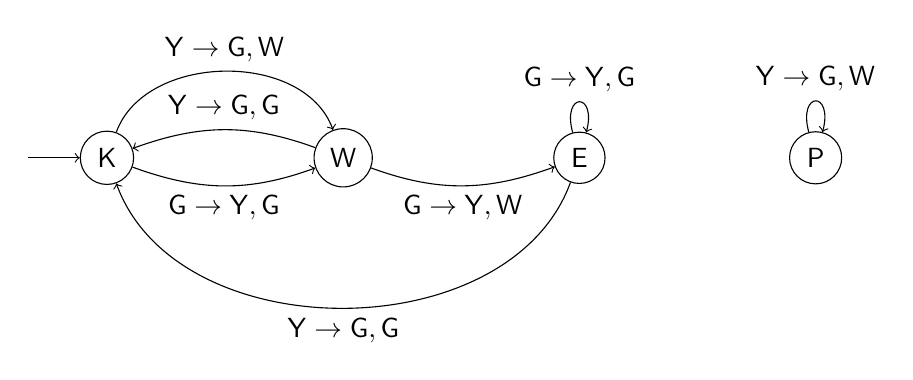
\begin{tikzpicture}
\node[draw, circle] (K) at (0, 0) {\sffamily K};
\node[draw, circle] (W) at (3, 0) {\sffamily W};
\node[draw, circle] (E) at (6, 0) {\sffamily E};
\node[draw, circle] (P) at (9, 0) {\sffamily P};
\draw[->] (-1, 0) to (K);
\draw[->] (E) to[out=-110, in=-70] node[midway, below] {$\q{Y} \rightarrow \q{G}, \q{G}$} (K);
\draw[->] (K) to[out=70, in=110] node[midway, above] {$\q{Y} \rightarrow \q{G}, \q{W}$} (W);
\draw[->] (K) to[out=-20, in=-160] node[midway, below] {$\q{G} \rightarrow \q{Y}, \q{G}$} (W);
\draw[->] (W) to[out=160, in=20] node[midway, above] {$\q{Y} \rightarrow \q{G}, \q{G}$} (K);
\draw[->] (W) to[out=-20, in=-160] node[midway, below] {$\q{G} \rightarrow \q{Y}, \q{W}$} (E);
\draw[->] (E) to[loop above] node[midway, above] {$\q{G} \rightarrow \q{Y}, \q{G}$} (E);
\draw[->] (P) to[loop above] node[midway, above] {$\q{Y} \rightarrow \q{G}, \q{W}$} (P);
\end{tikzpicture}

Only the same sources of redundancy in the full results appear in the
top five equivalence sets for Player 2. Player 1 appears to have an advantage
in the Platypus game as the best machine for Player 1 earns more wins than
the best machine for Player 2, but the best machine for Player 2 earns
more points. This may be due to the Platypus state being dead in all top 5
equivalence sets, so the machines will never attempt to halt the game.
\chapter{Conclusion}

The full Platypus tournament was originally speculated to be infeasible to
run, but I have completed in 9 days by detecting equivalent machines and
then using a fast interpreter for the remaining matches.

Simple algorithms suffice to detect many equivalent machines: dead
code elimination determines that three fifths of all possible Platypus
machines are redundant, and additionally renaming the Emu and
Wombat states of a machine makes four fifths of all Platpypus machines
redundant. A more complex algorithm like an adaptation of DFA
minimisation has diminishing returns, but stills help to reduce the
number of remaining matches (which is quadratic to the number of
remaining machines).

While equivalence detection is much faster than running all of the
remaining matches, faster equivalence detection allows for faster
experimentation with detection algorithms, and speeds up finding
counter-examples which were invaluable while testing new algorithms.
The equivalence detection can be parallelised across multiple threads,
and DFA minimisation for small machines like Platypus machines
can further be sped up using a data-parallel algorithm.

The Platypus tournament can be parallelised over multiple threads of a
modern CPU, multiple lanes of single instruction-multiple data extensions,
and the many lanes of GPUs, and over multiple computers. But care must
be taken to avoid communicating all the results, as the atomic operations
required to record a result of a match can take more time than running
the match on large CPUs and GPUs; a distributed Platypus tournament
similarly must avoid being bottlenecked by network latency when recording
the results of many matches.

\section{Future directions}

The results suggest that we could reduce the time taken to run full
tournaments of similar games by considering equivalences at a higher
level of abstraction. For example, some machines will perform identically
in a tournament while not behaving identically in each individual match,
as I found for flipping directions in the Platypus game. More redundancy
can be found by considering the possible behaviours of individual players in a
multi-player game, as I found for the first player in the Platypus game.

Further analysis of the results would be interesting, as I have only presented
patterns in the top 10 machines of the full tournament and in the top 5
machines for either player. I did not cover any trends or distributions within
across all the machines; one could find the performance of machines with
particular properties, such as if the Platypus state is reachable and thus the
machine may halt the game.

The results would also be useful to measure the accuracy of running
competitions between machines with different structures. Such competitions
involve fewer matches but might be less accurate, trading time for precision.
The rankings from the full tournament could be compared to the rankings
from some other competition to determine the accuracy of the competition.

The interpreters and efficient representation require some tricky coding to
implement, which at best requires more effort from researchers to get high
performance, and at worst deters researchers from investigating similar
games. Such deterrance could be reduced by tools to generate efficient
representations and interpreters from less tricky specifications. Tools
already exist for compiling specifications of custom representations of
algebraic data types \cite{bit-stealing}, for converting interpreters
into compilers \cite{meta-compilation}, and for automatically porting
code written for CPUs to run on GPUs \cite{gpu-first}, which may all
be relevant.

\printbibliography

\end{document}

%%% Local Variables: 
%%% coding: utf-8
%%% mode: latex
%%% TeX-engine: xetex
%%% End: 
